%%%%%%%%%%%%%%%%%%%%%%%%%%%%%%%%%%%%%%%%%
% FRI Data Science_report LaTeX Template
% Version 1.0 (28/1/2020)
%
% Jure Demšar (jure.demsar@fri.uni-lj.si)
%
% Based on MicromouseSymp article template by:
% Mathias Legrand (legrand.mathias@gmail.com)
% With extensive modifications by:
% Antonio Valente (antonio.luis.valente@gmail.com)
%
% License:
% CC BY-NC-SA 3.0 (http://creativecommons.org/licenses/by-nc-sa/3.0/)
%
%%%%%%%%%%%%%%%%%%%%%%%%%%%%%%%%%%%%%%%%%


%----------------------------------------------------------------------------------------
%	PACKAGES AND OTHER DOCUMENT CONFIGURATIONS
%----------------------------------------------------------------------------------------
\documentclass[fleqn,moreauthors,10pt]{ds_report}
\usepackage[russian,english]{babel}
\usepackage[T2A,T1]{fontenc}
\usepackage{amsmath}

\graphicspath{{fig/}}

\usepackage{multirow}
\usepackage{hhline}
\usepackage{makecell}
\usepackage{array}

\usepackage{color, colortbl}
\definecolor{Blue}{rgb}{0.8549,0.9098,0.9882}
\definecolor{Red}{rgb}{0.9725,0.8078,0.8}


%----------------------------------------------------------------------------------------
%	ARTICLE INFORMATION
%----------------------------------------------------------------------------------------

% Header
\JournalInfo{FRI Natural language processing course 2024}

% Interim or final report
\Archive{Project report}
%\Archive{Final report}

% Article title
\PaperTitle{Unsupervised Domain Adaptation for Sentence Classification}

% Authors (student competitors) and their info
\Authors{Karmen Frank, Veronika Matek and Luka Mihelič}

% Advisors
\affiliation{\textit{Advisors: Boshko Koloski, Aleš Žagar, Slavko Žitnik}}

% Keywords
\Keywords{Domain Adaptation, TSDAE, GPL, SBERT, Sentiment Classification}
\newcommand{\keywordname}{Keywords}


%----------------------------------------------------------------------------------------
%	ABSTRACT
%----------------------------------------------------------------------------------------

\Abstract{
Methods like SBERT are used for deriving sentence embeddings, but often do not perform well on more specific domains. This problem might be avoided if the chosen base model is fine-tuned using unsupervised fine-tuning methods like TSDAE~\cite{wang-etal-2021-tsdae-using} and GPL~\cite{GPL}. The two stated methods were used to fine-tune two base models, first {\it paraphrase-multilingual-MiniLM-L12-v2}~\cite{reimers-2019-sentence-bert} model and then the Slovenian {\it SloBERTa}~\cite{sloberta} model. Fine-tuning was conducted on the two base models using various versions of TSDAE and GPL methods, leading to the creation of multiple model variants. To be able to evaluate the obtained models on the sentiment classification problem, we also implemented a simple classifier neural network. The {\it SloBERTa} model fine-tuned with the TSDAE method achieved the best F1 score on the SentiNews dataset~\cite{sentiNews}, with the raw {\it SloBERTa} following close by.
}

%----------------------------------------------------------------------------------------

\begin{document}

% Makes all text pages the same height
\flushbottom

% Print the title and abstract box
\maketitle

% Removes page numbering from the first page
\thispagestyle{empty}

%----------------------------------------------------------------------------------------
%	ARTICLE CONTENTS
%----------------------------------------------------------------------------------------

\section*{Introduction}

\iffalse
	In the Introduction section you should write about the
	relevance of your work (what is the purpose of the project,
	what will we solve) and about related work (what solutions
	for the problem already exist). Where appropriate, reference
	scientific work conducted by other researchers.
\fi

Previous state-of-the-art methods, like SBERT, for deriving sentence embeddings have a key problem of not working for specific topics and domains. We bypass this problem by additionally fine-tuning our non-domain-specific base model using methods like TSDAE and GPL. Both of the methods have been proven to significantly outperform previous state-of-the-art models, like Masked Language Model, on domain specific training data, working even better if combined together~\cite{wang-etal-2021-tsdae-using, GPL}.

Most of these previous successful methods were trained on Semantic Textual Similarity, which does not take into account any domain knowledge. Some examples of these approaches are SBERT and Infersent. One such reason for the lack of domain knowledge is that training a model might require a lot of labeled data, which can be expensive and hard to get. This holds true especially for specific topics. One way of solving this is training the model on the general corpus before fine-tuning it to the required domain~\cite{wang-etal-2021-tsdae-using, GPL}.

In this report we aim to fine-tune an unsupervised multilingual base model with SBERT architecture with two of the mentioned domain adaptation techniques, namely Transformer-based Sequential Denoising Auto-Encoder (TSDAE) and Generative Pseudo Labeling (GPL) on the SentiNews classification dataset. We classify Slovenian sentences based on their sentiment, which can be positive, neutral or negative. We compare the results given by the pretrained base model and by the base model fine-tuned with both mentioned methods and combinations of the two.

We observe any improvement when faced with domain specific data compared to SBERT, trained on the exact same input sentences. We also distinguish the impact of different parameters during the learning of each approach and try to find the optimums.



%------------------------------------------------



\section*{Methods}

\iffalse
Use the Methods section to describe what you did an how you did it -- in what way did you prepare the data, what algorithms did you use, how did you test various solutions ... Provide all the required details for a reproduction of your work.
\fi

\subsection*{SBERT}
SBERT (Sentence Bidirectional Encoder Representations from Transformers) adds siamese and triplet structure networks to the pre-trained transformer network BERT, which produces state-of-the-art results for natural language processing tasks such as sentence classification, question answering and sentence-pair regression. SBERT applies a pooling layer to the output of a BERT/RoBERTa model, deriving fixed sized sentence embeddings. With the added network structures we can fine-tune the model and update weights so the output results are sentence embeddings that are semantically meaningful~\cite{SBERT}.

Semantic aspects embedded in the continuous vector space can be measured with the cosine metric similarity, where similar semantic representations in a high-dimensional vector space are closer to each other. The available training data for a given knowledge domain also defines the SBERT network structure. Therefore we may use the classification, regression or the triplet objective function for different kind of tasks.

The classification objective function concatenates sentence embeddings \(u\) and \(v\) with the element-wise difference \(|u - v|\) and multiplies it with the trainable weight \( W_t \in \mathbb{R}^{3n \times k} \) \cite{SBERT}:

\begin{equation}
\begin{gathered}
o = \text{softmax}(W_t(u, v, |u - v|)) \text{,}
\end{gathered}
\label{eq:softmax}
\end{equation}

where $n$ is the sentence embeddings' dimension and $k$ number of labels.


\subsection*{TSDAE}

Transformer-based Sequential Denoising Auto-Encoder (TSDAE) is a state-of-the-art unsupervised method used for domain adaptation with an encoder-decoder architecture. A shortcoming of previous sentence embedding techniques like SBERT is the lack of domain knowledge. Fine-tuning a model like this with TSDAE can adapt our model to a specific domain without any labeled data, as this is hard and expensive to acquire~\cite{wang-etal-2021-tsdae-using}.

Before training the model, TSDAE corrupts the input sentences, for example by deleting or swapping words, and encodes them to a fixed size vector. The goal of the decoder is to reconstruct the vectors of the original input by predicting what was changed. It is important to note that the decoder has no context as it doesn't have access to other sentence embeddings and thus creates a bottleneck~\cite{wang-etal-2021-tsdae-using}. This architecture can be seen in Figure~\ref{fig:tsdae}.

\begin{figure}[ht]\centering
	\vspace{12 pt}
	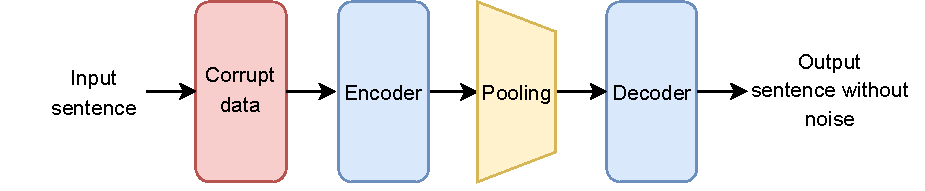
\includegraphics[width=\linewidth]{TSDAE_scheme.pdf}
	\vspace{5 pt}
	\caption{Workflow of TSDAE. The input sentences are first corrupted and then encoded into fixed size vectors. The vectors are pooled and then attempted to be reconstructed with the decoder.}
	\label{fig:tsdae}
\end{figure}

For the purpose of classifying Slovenian sentences based on their sentiment we fine-tune the SBERT model with TSDAE. During training we use the DenoisingAutoEncoderLoss as our loss function, which expects pairs of original and corrupted sentences as the input. We train the model where the decoder attempts the reconstruction of the corrupted sentences and compare our results with the corpus~\cite{SentenceTransformers}.

% TSDAE has been shown by Wang, Reimers and Gurevych \cite{wang-etal-2021-tsdae-using} to outperform other unsupervised approaches and other supervised models, trained with a lot of labeled data. Many previous works were evaluated on Semantic Textual Similarity (STS) which might return good performance but it is unclear how it performs on specific domains \cite{wang-etal-2021-tsdae-using}.


\subsection*{GPL}

The Generative Pseudo Labeling (GPL) is a domain adaptation technique that utilizes unsupervised learning. It allows us to fine-tune a dense retrieval model (in our case SBERT \cite{SBERT}) on a desired domain. First step of GPL is preparing (query, sentence)-pairs. This takes three phases: generating suitable queries, negative mining and using cross-encoder to assign a score to each pair \cite{GPL}. This process is visualised in Figure~\ref{fig:GPL}.

\begin{figure}[ht]\centering
	\vspace{12 pt}
	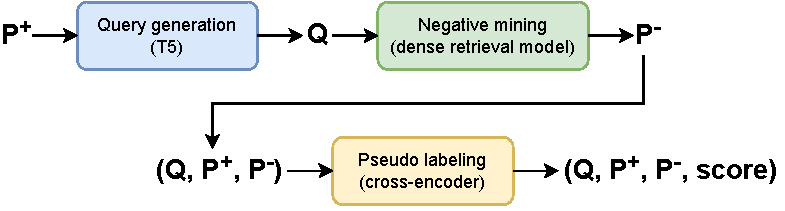
\includegraphics[width=\linewidth]{GPL_data_preprocessing.pdf}
	\vspace{5 pt}
	\caption{The workflow of GPL's sentence preparation step. Queries $Q$ are generated for each input sentence $P^{+}$. The generated queries are then used for negative mining or finding similar sentences $P^{-}$. Pseudo labeling step involves a cross-encoder that assigns a score to each (query, sentence)-pair.}
	\label{fig:GPL}
\end{figure}

Queries are generated using a pretrained T5 encoder-decoder model \cite{T5}. Three queries are generated for each input sentence. The next step is negative mining, where 50 of the most similar sentences are retrieved for each of the generated queries, using an existing dense retrieval model. The (query, input sentence)-pairs are denoted as $(Q, P^{+})$ and the negative sentence as $P^{-}$.

The last step of data preparation involves a cross-encoder that assigns a score to each (query, sentence)-pair. For each $(Q, P^{+}, P^{-})$-tuple a margin $\delta$ is calculated using the next equation:
\begin{equation}
	\delta = \text{CE}(Q, P^{+}) - \text{CE}(Q, P^{-})\text{,}
\label{eq:delta}
\end{equation}
where $CE$ is the score predicted by the cross-encoder. This gives us a dataset $D_{GPL} = {\{ ( Q_i, P_i, P_i^{-}, \delta_i ) \}}_i$, which is used for training a dense retrieval model with the MarginMSE loss function. This model thus learns to map queries and sentences into a vector space and is fine-tuned to a given domain.

The MarginMSE loss \cite{marginMSE} relies on the scores, or pseudo labels, provided by the cross-encoder. It teaches the dense retrieval model to predict the margin between the score of $(Q, P^{+})$-pair and score of $(Q, P^{-})$-pair. It follows the next equation:
\begin{equation}
	\text{MarginMSE} = \frac{1}{N} \sum_{i=0}^{N-1} |\hat{\delta_i} - \delta_i|^{2} \text{,}
\label{eq:margin}
\end{equation}
where $N$ is the batch size, $\delta_i$ is defined in equation~\ref{eq:delta}, provided by the cross-encoder, and $\hat{\delta_i}$ is derived by the (student) dense retrieval model, which we are fine-tuning.


%------------------------------------------------



\section*{Experiments}
%TODO -> SBERT?
The experiments were conducted on two different sentence-transformer (SBERT architecture) base models, the first one being multilingual {\it paraphrase-multilingual-MiniLM-L12-v2}~\cite{reimers-2019-sentence-bert} and the second Slovenian {\it SloBERTa}~\cite{sloberta}. Both models were individually fine-tuned with the TSDAE and GPL method as well as a combination of TSDAE+GPL.

We used the SentiNews dataset \cite{sentiNews}, which contains 169k sentences from 10.4k documents, equiped with sentiment labels, in the Slovenian language. The sentiment labels can be neutral, negative or positive. A few examples of dataset's elements are shown in Table~\ref{tab1}.

\begin{table}[!h]
	\footnotesize
	\begin{center}
		\begin{tabular}{ |l|c| }
		\hline
		\rowcolor{Blue}Sentence & Sentiment \\
		\hline

		Kaže, da se blejskim vilam vendarle obeta lepša prihodnost. & positive\\
		O tem bo Evropska komisija odločala septembra. & neutral\\
		V Sloveniji je ta rast znašala sedem odstotkov. & negative\\

		\hline
		\end{tabular}
	\end{center}
\caption{Examples from the SentiNews dataset \cite{sentiNews}.}
\label{tab1}
\end{table}

The dataset was split into train (70\%), validation (10\%) and test set (20\%). For each method we use to fine-tune the base model, the exact same datasets are used.

The approaches were tested on the test set and evaluated using the F1 score that combines precision and recall. It is defined by the following equation:
\begin{equation}
	\text{F1 score} =\frac{2 \times \text{\it{precision}} \times \text{\it{recall}}}{\text{\it{precision}} + \text{\it{recall}}} \text{,}
\label{eq:f1}
\end{equation}
where precision and recall are defined as:
\begin{equation}
	\text{precision} =\frac {\text{TP}}{\text{TP} + \text{FP}} \text{,}
\label{eq:precision}
\end{equation}
\begin{equation}
	\text{recall} =\frac {\text{TP}}{\text{TP} + \text{FN}} \text{.}
\label{eq:recall}
\end{equation}

Precision metric of the model tells us how many accurate positive predictions have been made based on the equation \ref{eq:precision} and recall how well the model covered all true positives from the positive sample set as shown in equation \ref{eq:recall}. The F1 score is a relative metric that tells us how well our chosen model extracts sentiment polarity from semantics and shows overall performance for each possible sentiment class triplet.



\subsection*{Classifier}

To be able to test the base model and its fine-tuned variants on the sentiment classification problem, we prepared a simple classifier. The classifier takes a sentence encoding of length 384 (or 768 if the base model is {\it SloBERTa}) and transforms it into a vector of size 3 - the number of classes in our classification problem. The transformation is done via a trainable linear layer. Softmax is used on this vector to obtain probabilities for each of the classes and as the output of the classifier model the class with the highest probability is returned.

For each model that we evaluated, a new classifier was trained. All of the classifiers were trained on the same training set and used the same validation set. Data was split into batches of size 32, we used learning rate 0.001 with the Adam optimizer and trained the classifier for 10 epochs. The classifier model with the highest F1 score on the validation set was chosen.


\subsection*{TSDAE}

For TSDAE fine-tuning we first prepare our dataset split and then select our base model.
We choose a sentence-transformer model {\it paraphrase-multilingual-MiniLM-L12-v2} as our starting point of training, which maps sentences to 384 dimensional vectors or sentence encodings. The second base model SloBERTa was also fine-tuned using this approach, but instead returns 768 dimensional embeddings.

We take the training data of our split dataset and corrupt the sentences by removing words using the {\it DenoisingAutoEncoderDataset}. This function is used in combination with {\it DenoisingAutoEncoderLoss} which tries to reconstruct the sentences without noise.

We train the model using batch size 32, 10 epochs and learning rate of 3e-5. We then train a classifier to predict sentiment from the 384-dimensional vectors (or 768 for SloBERTa). We calculate the precision, recall and F1 score on the test dataset.


\subsection*{GPL}
The fine-tuning with the GPL method consisted of training two versions. Each one was fine-tuned using a different T5 model for query qeneration. The training dataset of the first T5 model did not include the Slovene language, this model is also known as {\it msmarco-14langs-mt5-base-v1}~\cite{msmarco14langs}. The second choice for the T5 model is made specifically for the Slovene language and producing Slovene queries, this is the {\it slv\_doc2query}~\cite{boshko} transformer model.

We train the model for 140,000 steps, with the batch size set to 32, generating 3 queries per sentence and 50 negative examples per query. For the score evaluation method for dense vector retrieval we use computation of cosine similarity, which also works for usage of the default hybrid retriever in combination of {\it msmarco-distilbert-base-v3 }~\cite{msmarcodistil} and {\it msmarco-MiniLM-L-6-v3}~\cite{msmarcominilm} for negative mining. After fine-tuning the chosen base model with the GPL, we train a classifier that receives as input 384-dimensional vector embedding (or 768 in the case of SloBERTa) and returns the sentiment classification. The results are evaluated in the same way as the base models and TSDAE fine-tuned models.


%------------------------------------------------



\section*{Results}

% Use the results section to present the final results of your work. Present the results in a objective and scientific fashion. Use visualisations to convey your results in a clear and efficient manner. When comparing results between various techniques use appropriate statistical methodology.

\subsection*{\large{1. Paraphrase-multilingual-MiniLM}}

The fine-tuning and evaluation was first executed on the {\it paraphrase-multilingual-MiniLM-L12-v2}~\cite{reimers-2019-sentence-bert} model. The compared models in this section were:
\begin{itemize}
	\item base model {\it paraphrase-multilingual-MiniLM-L12-v2},
	\item base model fine-tuned with the TSDAE method, trained for 5 epochs - denoted as $\text{TSDAE}^{5}$,
	\item base model fine-tuned with the TSDAE method, trained for 10 epochs - denoted as TSDAE,
	\item base model fine-tuned with the TSDAE method, trained for 15 epochs - denoted as $\text{TSDAE}^{15}$,
	\item base model fine-tuned with the GPL method and {\it msmarco-14langs-mt5-base-v1} \cite{msmarco14langs} for the T5 model - denoted as GPL and
	\item base model fine-tuned with the GPL method and \\{\it slv\_doc2query}~\cite{boshko} for the T5 model - denoted as $\text{GPL}_{SLO}$.
\end{itemize}

A new classifier was trained with the same parameters for each of the stated models. They were evaluated on the test set part of the SentiNews dataset~\cite{sentiNews}. The results are presented in Table~\ref{tab2}.

\begin{table}[!h]
	\footnotesize
	\begin{center}
		\begin{tabular}{ |l|c|c|c| }
		\hline
		\rowcolor{Blue}Model & Precision & Recall & F1 score\\
		%\hhline{|=|=|=|=|}
		\hline

		Base model & 0.6124 & 0.6014 & \textbf{0.5637}\\
		\hline
		$\text{TSDAE}^{5}$ & 0.5682 & 0.5598 & 0.4968\\
		TSDAE &  0.5673 & 0.571 & \textbf{0.5257}\\
		$\text{TSDAE}^{15}$ & 0.567 & 0.5665 & 0.5142\\
		\hline
		GPL & 0.4651 & 0.5104 & 0.3857\\
		$\text{GPL}_{SLO}$ & 0.5641 & 0.5663 & \textbf{0.5125}\\

		\hline
		\end{tabular}
	\end{center}
\caption{Results of the base model and its fine-tuned variants on the SentiNews dataset~\cite{sentiNews}.}
\label{tab2}
\end{table}

We observe that both fine-tuned methods achieve lower F1 score than the base model, therefore perform worse on our sentiment classification problem. The highest F1 score, besides the base model, is attained with TSDAE fine-tuning using 10 epochs. Comparing all TSDAE models, we notice that training using 5 epochs is not a sufficient amount as the F1 score is slightly lower than training with 10 epochs and we assume the model does not learn as much. On the other hand, training with 15 epochs also achieves a lower score, but we assume this is due to the start of overfitting of our model.

For GPL fine-tuned models we observe that $\text{GPL}_{SLO}$ performs better than GPL in terms of the F1 score by 0.1268 or 32.88\%. This is because the T5 model used in GPL returns incomprehensible queries and in other languages than Slovenian,
since Slovenian was not a part of its training dataset. Because we are fine-tuning our model on Slovenian sentences, this T5 model is not ideal for our GPL fine-tuning. We proved this by using a T5 model {\it slv\_doc2query} which was trained only for the Slovenian language. We can compare the returned queries for both T5 models in Table \ref*{queries}.

\begin{table}[!h]
    \tiny
	\setlength{\tabcolsep}{5pt}
    \renewcommand{\arraystretch}{1.5}
    \begin{center}
        \begin{tabular}{ |c|c|c| }
        \hline
        \rowcolor{Blue}T5 model & Sentence & Queries \\
        \hline
        \multirow{3}{*}{\makecell{{\it msmarco-14langs-}\\{\it mt5-base-v1}}} & \multirow{3}{*}{\makecell{Bo evropska komisija \\ analizirala vzroke \\ rasti cen hrane.}} & \cellcolor{Blue}evroeuropeana komisija \\
         & & evro komisija \foreignlanguage{russian}{analizировала 'zogueность rastelaar'}?\\
         & & \cellcolor{Blue}bo europeana komisija \foreignlanguage{russian}{analizировала точки} \\
        \hline
        \multirow{3}{*}{{\it slv\_doc2query}} & \multirow{3}{*}{\makecell{Bo evropska komisija \\ analizirala vzroke \\ rasti cen hrane.}} & \cellcolor{Blue}Kateri je glavni vzrok za rast cen hrane? \\
         & & vzroki za rast cen hrane \\
         & & \cellcolor{Blue}Kaj povzroča rast cen hrane? \\
        \hline
        \end{tabular}
    \end{center}
    \caption{Examples of queries returned by each T5 model for the given sentence.}
    \label{queries}
\end{table}


\subsection*{Combining the methods}
Considering the results obtained in the GPL paper~\cite{GPL}, we decided to test a combination of the unsupervised adaptation techniques. The approach was to additionally fine-tune the TSDAE model with the GPL method with {\it slv\_doc2query} for the T5 model.


We also considered testing the approach of further fine-tuning the $\text{GPL}_{SLO}$ model using the TSDAE method for 10 epochs, but we were unable to do so as we could not resolve an error in time. Results of TSDAE+$\text{GPL}_{SLO}$, compared to the base model, are presented in Table~\ref{tab3}.

\begin{table}[!h]
	\footnotesize
	\begin{center}
		\begin{tabular}{ |l|c|c|c| }
		\hline
		\rowcolor{Blue}Model & Precision & Recall & F1 score\\
		\hline

		Base model & 0.6124 & 0.6014 & \textbf{0.5637}\\
		TSDAE+$\text{GPL}_{SLO}$ & 0.552 & 0.5555 & 0.496\\
		% $\text{GPL}_{SLO}$+TSDAE &  0.v & 0.v & 0.v\\

		\hline
		\end{tabular}
	\end{center}
\caption{Results of combining the fine-tuning methods TSDAE and GPL on the SentiNews dataset~\cite{sentiNews}.}
\label{tab3}
\end{table}

The F1 score of TSDAE+$\text{GPL}_{SLO}$ is lower than the value achieved by the base model for 0.0677 or 12.01\%. When checking the results stated in Table~\ref{tab2}, we also notice that the combination of the two unsupervised fine-tuning methods performs worse than if the methods are used individually. Compared to TSDAE, the decrease in F1 score is 0.0297 or 5.65\%, while compared to $\text{GPL}_{SLO}$ the decrease is 0.0165 or 3.22\%. The worsened performance is most likely because of the $\text{GPL}_{SLO}$ model overfitting on the training dataset.


\subsection*{Intermediate models in GPL}
\label{intermediate-paraphrase}
Since we used the \textit{gpl}\footnote{https://pypi.org/project/gpl/} library for fine-tuning a chosen model with the GPL method, it allowed us to save intermediate models during this process. The GPL method fine-tunes the model for 140,000 steps by default and saves a model every 10,000 steps. Thus we obtained 13 intermediate and 1 final model. We trained a classifier for each of the models and evaluated them on the train and test set parts of the SentiNews dataset~\cite{sentiNews}. The results\footnote{The results might not match the ones presented in Table~\ref{tab2}, since completely new classifiers were trained for this visualisation.} were plotted and are shown in Figure~\ref{fig:gpl-versions-train} and Figure~\ref{fig:gpl-versions} for GPL and in Figure~\ref{fig:gpl-slo-versions-train} and Figure~\ref{fig:gpl-slo-versions} for $\text{GPL}_{SLO}$.

\begin{figure}[h]
    \centering
    \begin{minipage}{0.5\textwidth}
        \centering
        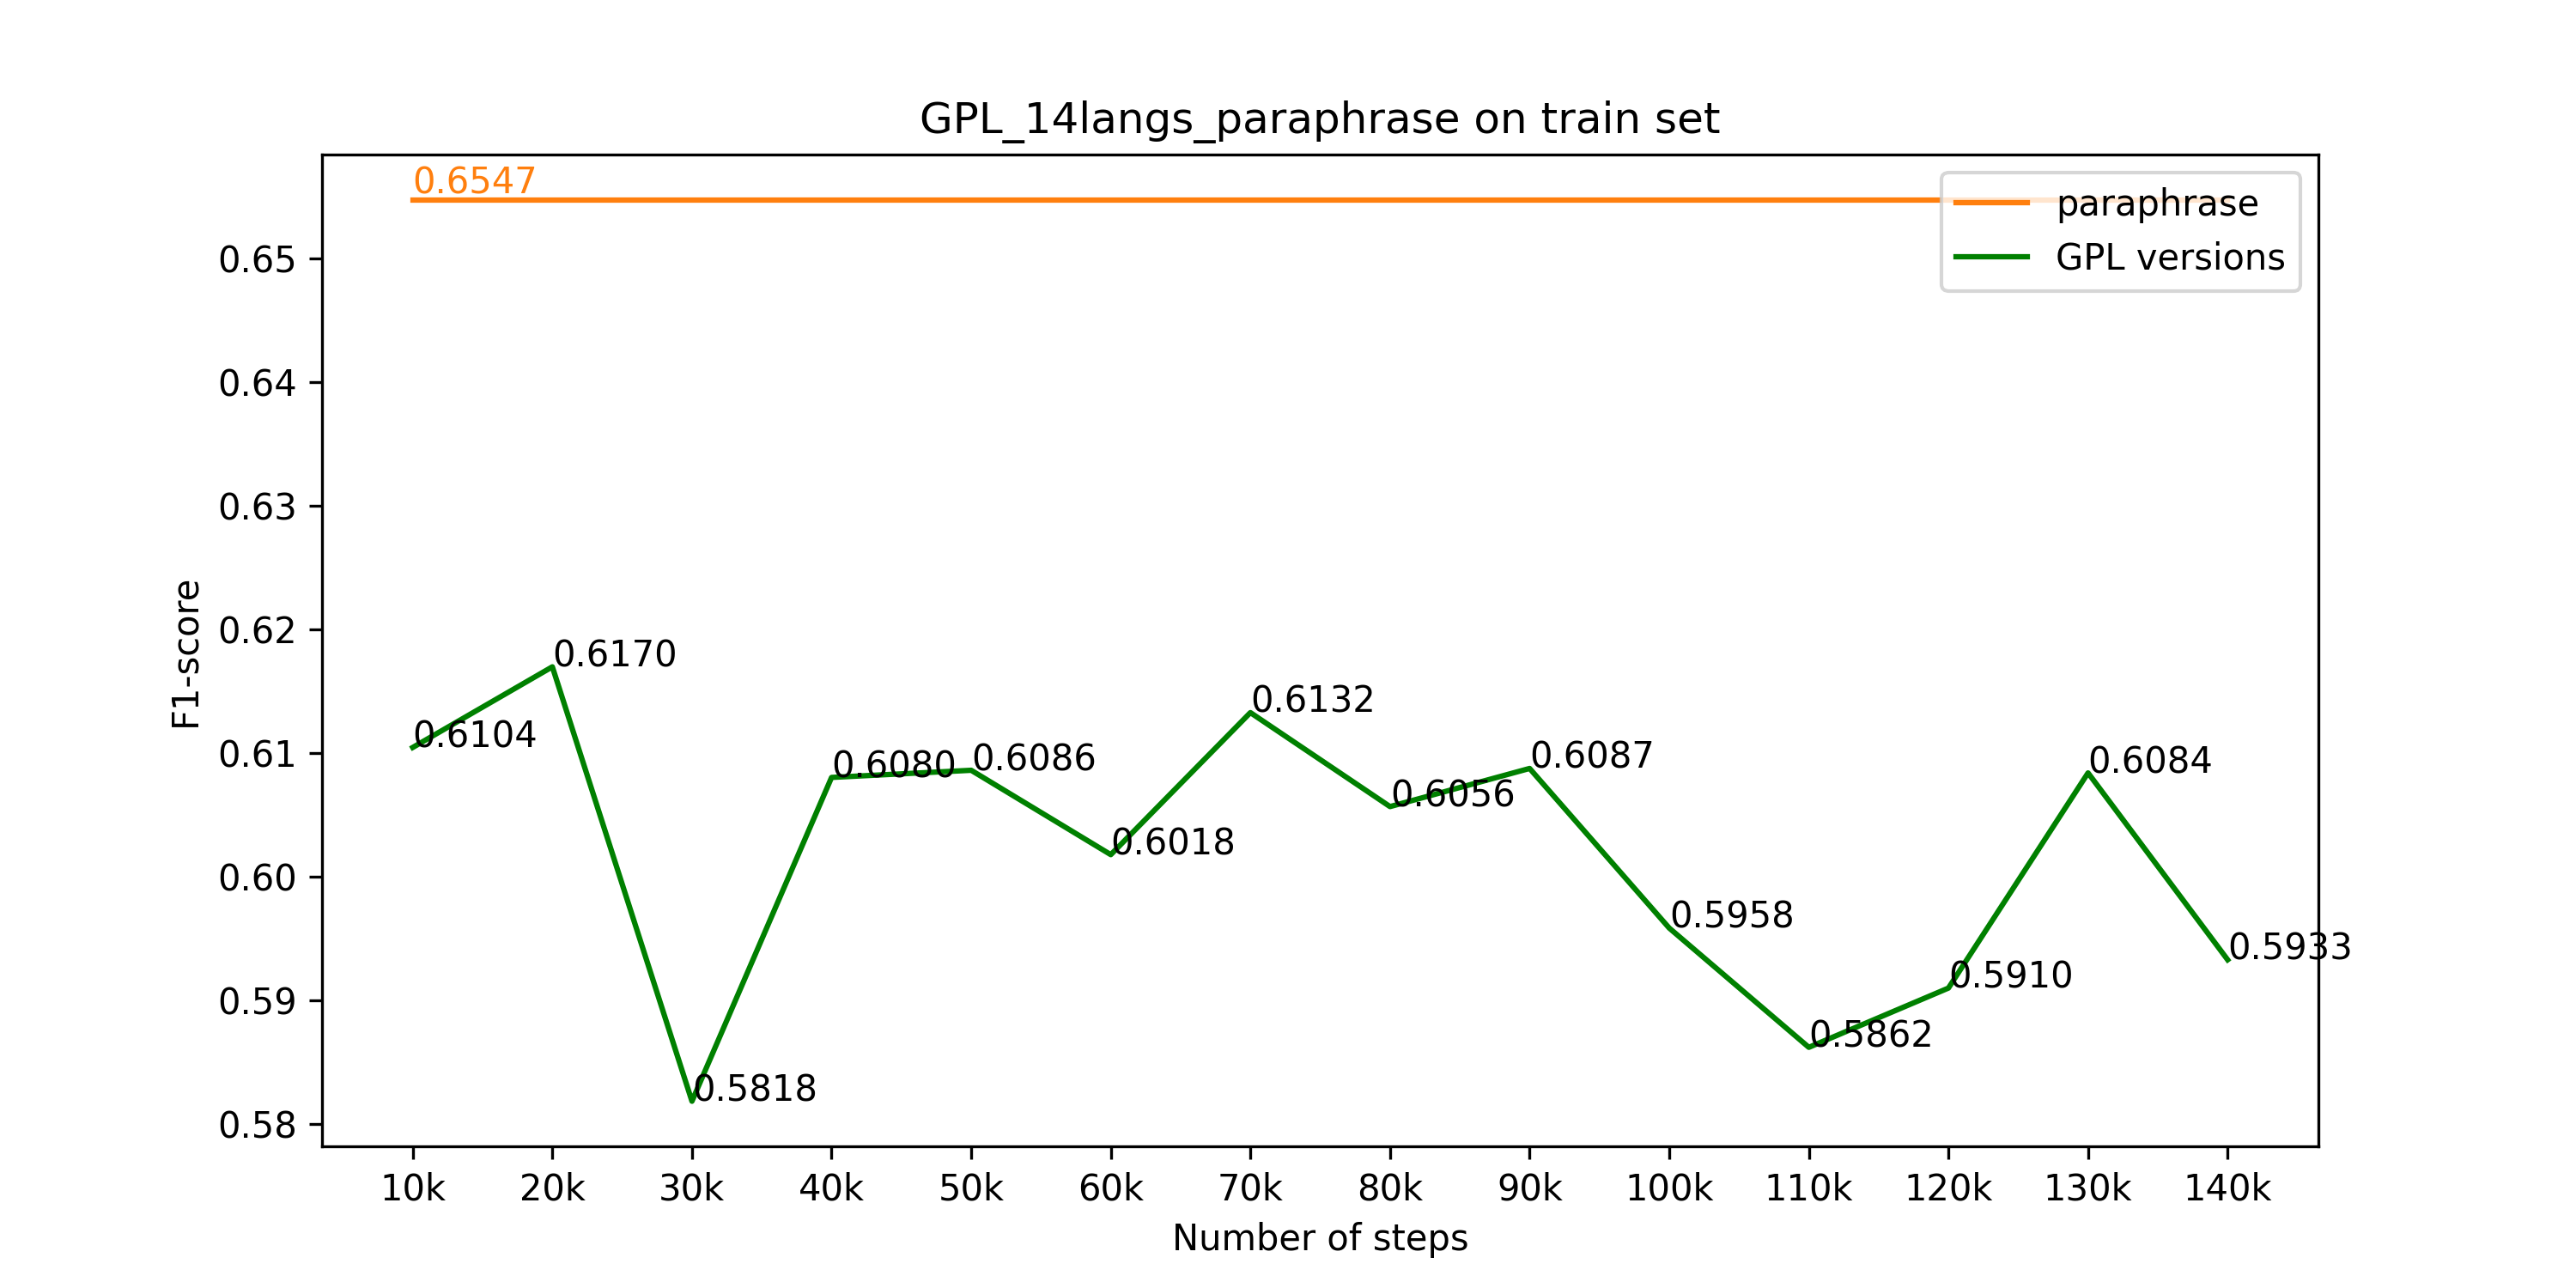
\includegraphics[width=\linewidth]{graphs/GPL_14langs_paraphrase_train.png}
        \caption{F1 score on \textit{train} set evaluated on models, obtained during fine-tuning with the GPL method with {\it msmarco-14langs-mt5-base-v1} \cite{msmarco14langs} for the T5 model.}
		\label{fig:gpl-versions-train}
    \end{minipage}\hfill
    \begin{minipage}{0.5\textwidth}
        \centering
        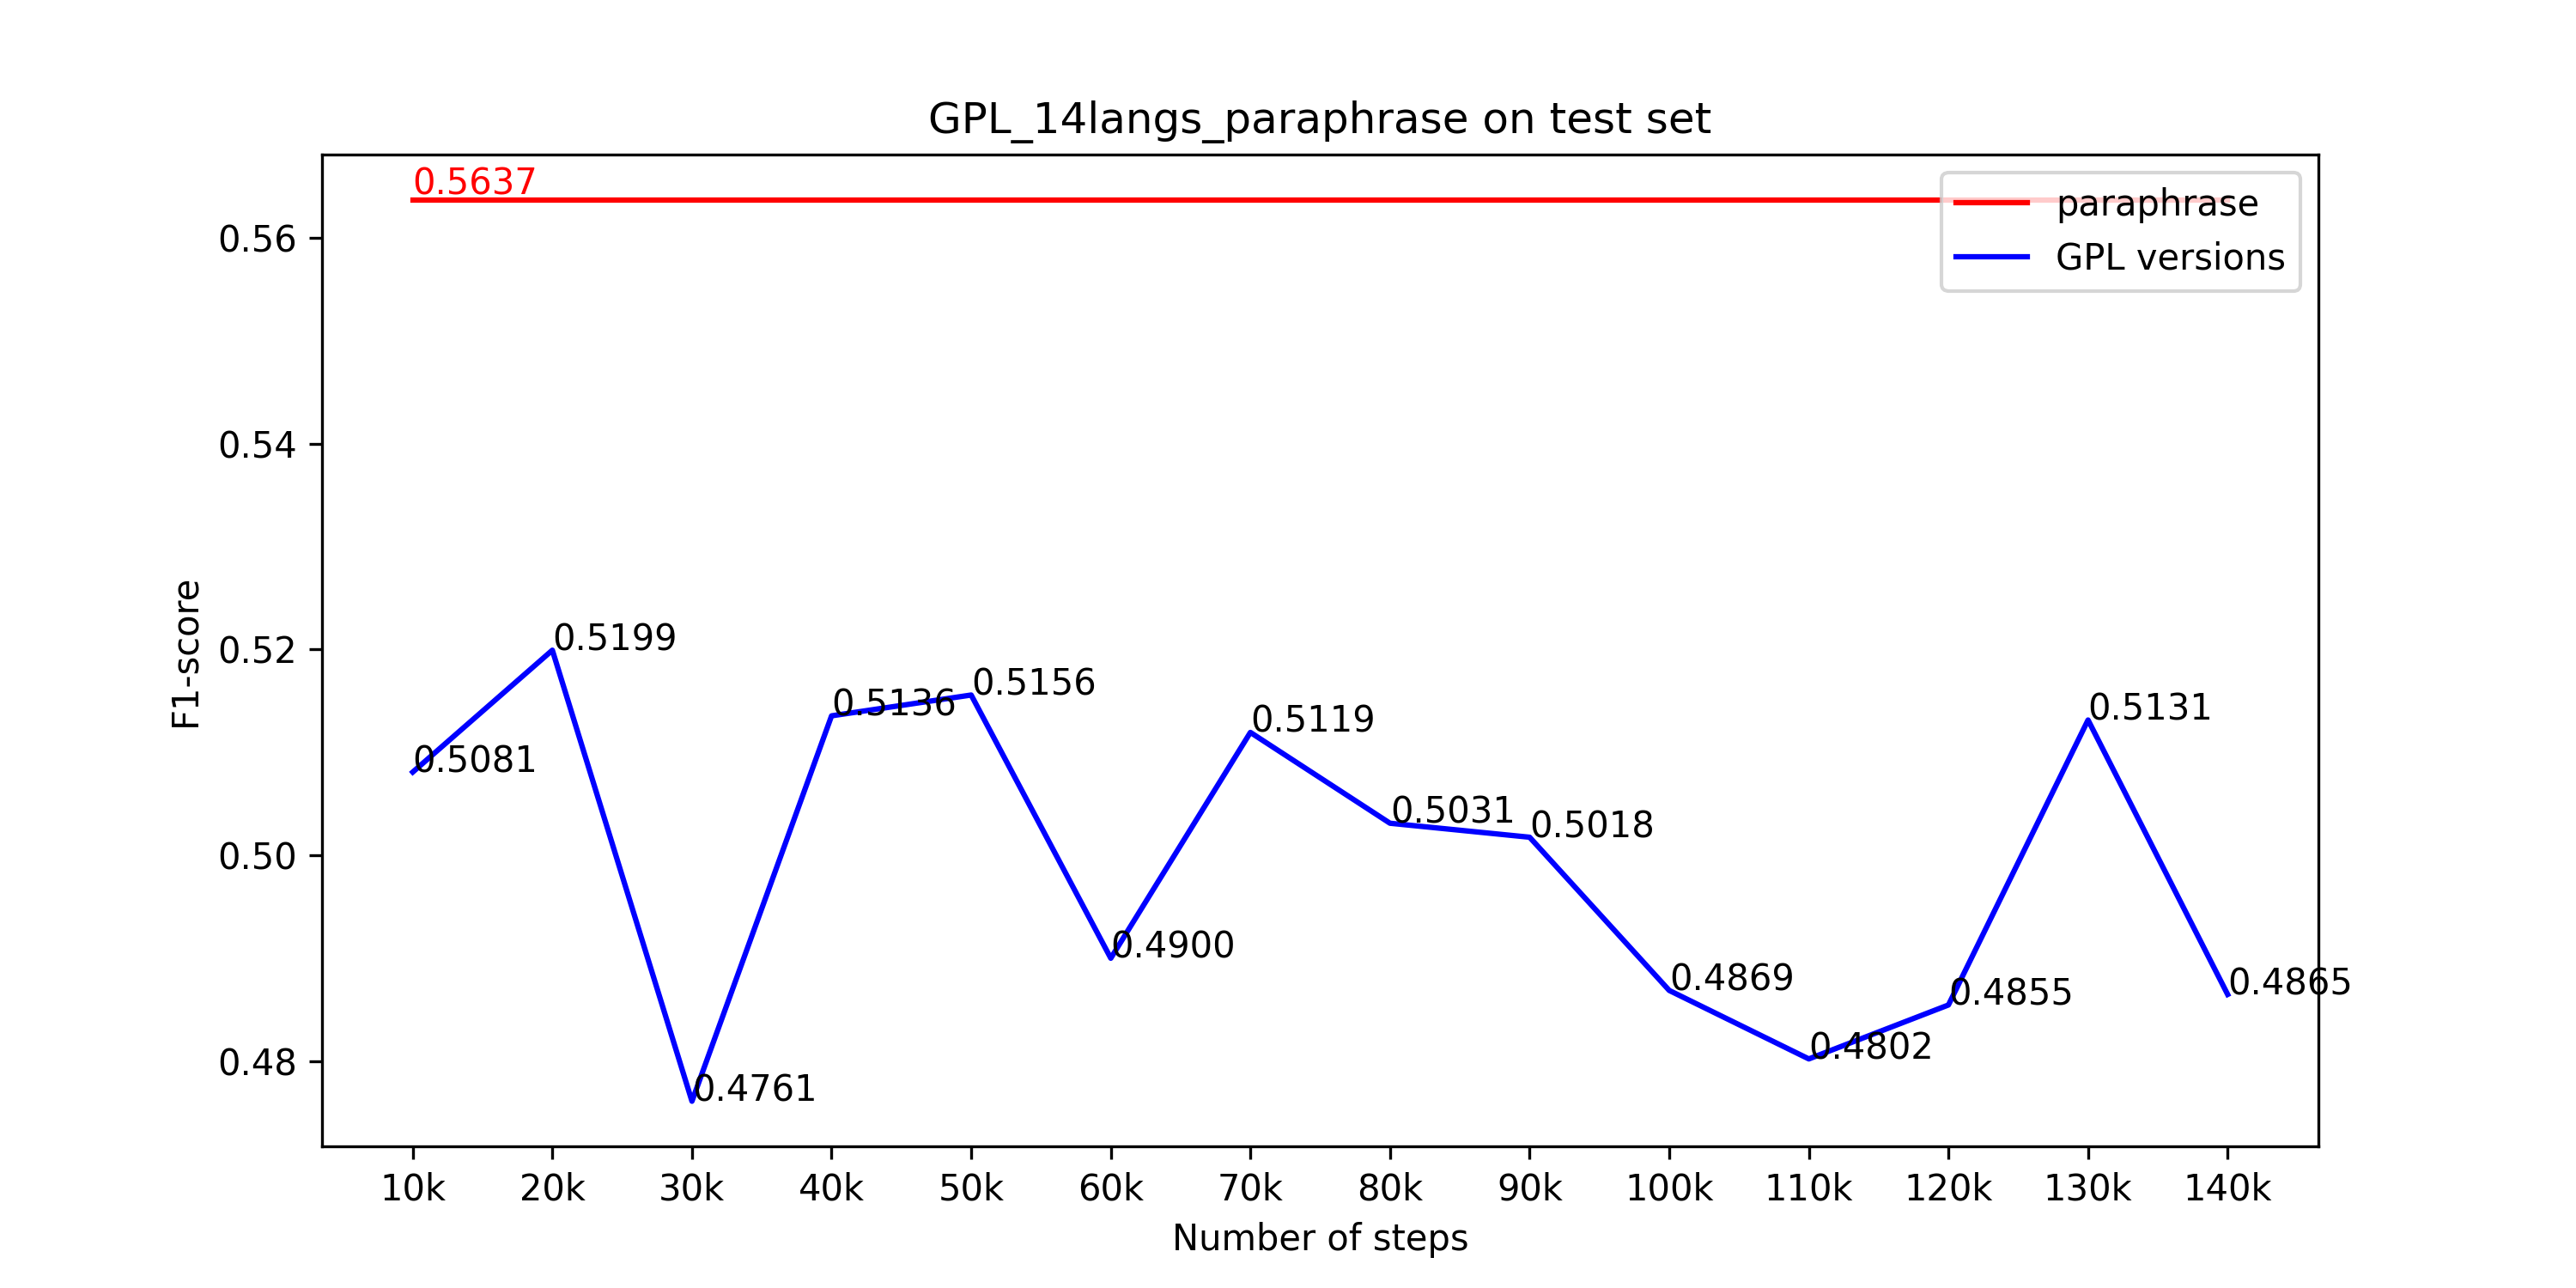
\includegraphics[width=\linewidth]{graphs/GPL_14langs_paraphrase_test.png}
        \caption{F1 score on \textit{test} set evaluated on models, obtained during fine-tuning with the GPL method with {\it msmarco-14langs-mt5-base-v1} \cite{msmarco14langs} for the T5 model.}
		\label{fig:gpl-versions}
    \end{minipage}
\end{figure}

\begin{figure}
    \centering
    \begin{minipage}{0.5\textwidth}
        \centering
        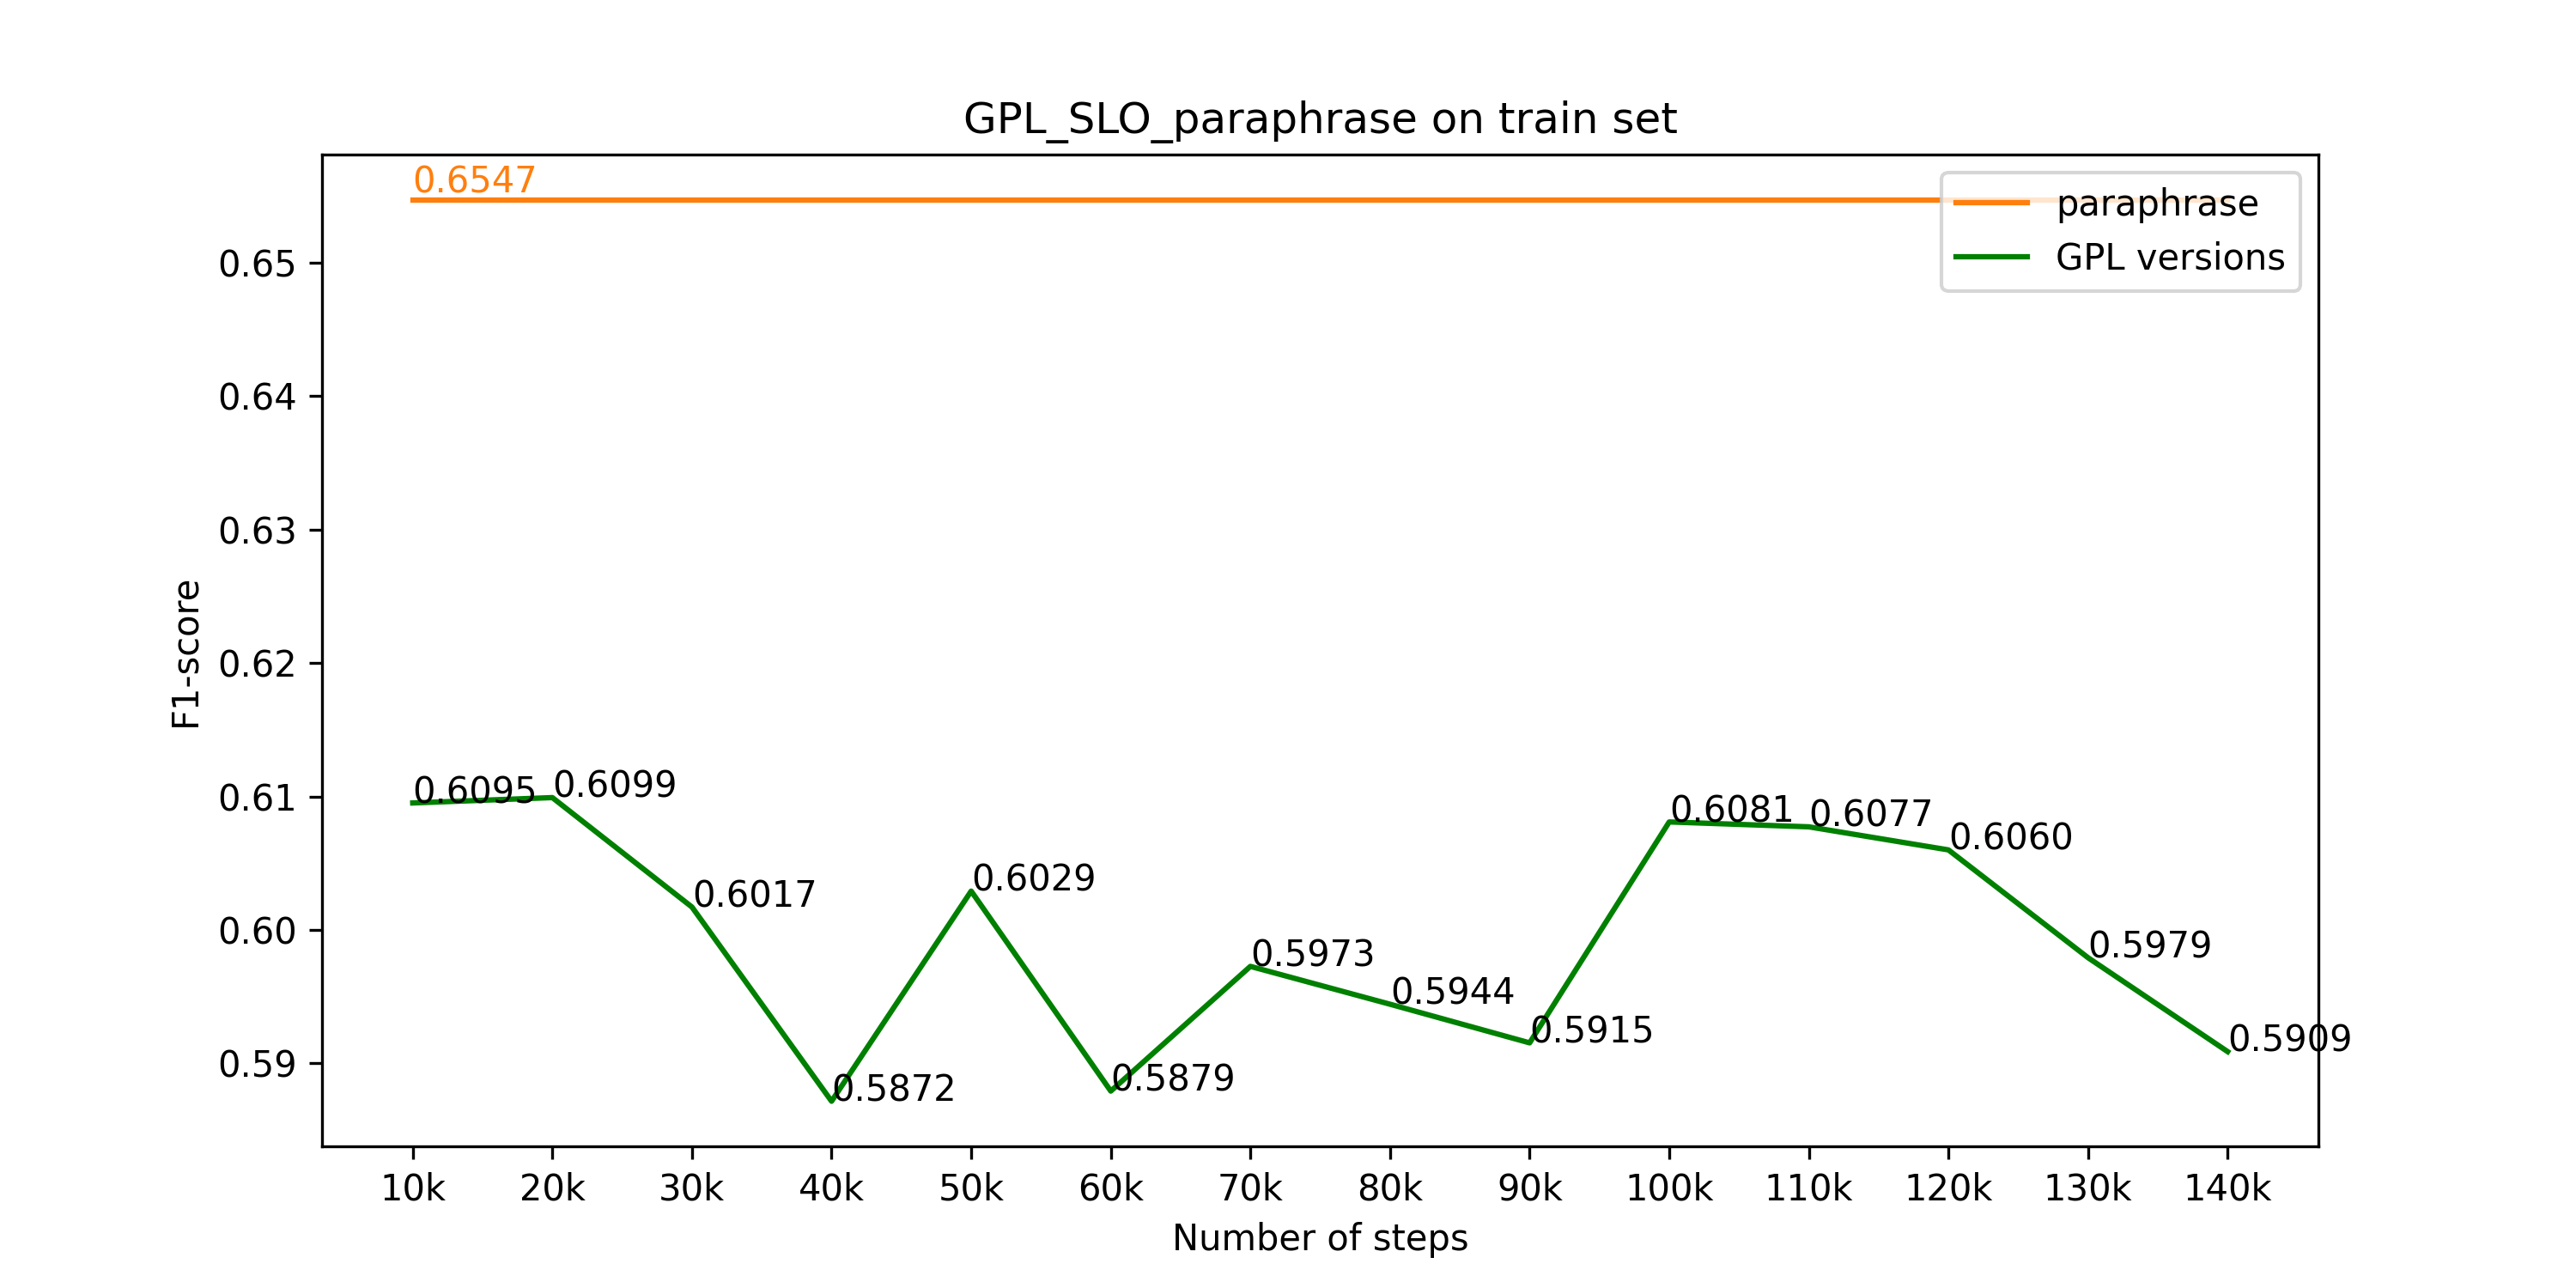
\includegraphics[width=\linewidth]{graphs/GPL_SLO_paraphrase_train.png}
        \caption{F1 score on \textit{train} set evaluated on models, obtained during fine-tuning with the GPL method with {\it slv\_doc2query}~\cite{boshko} for the T5 model.}
		\label{fig:gpl-slo-versions-train}
    \end{minipage}\hfill
    \begin{minipage}{0.5\textwidth}
        \centering
        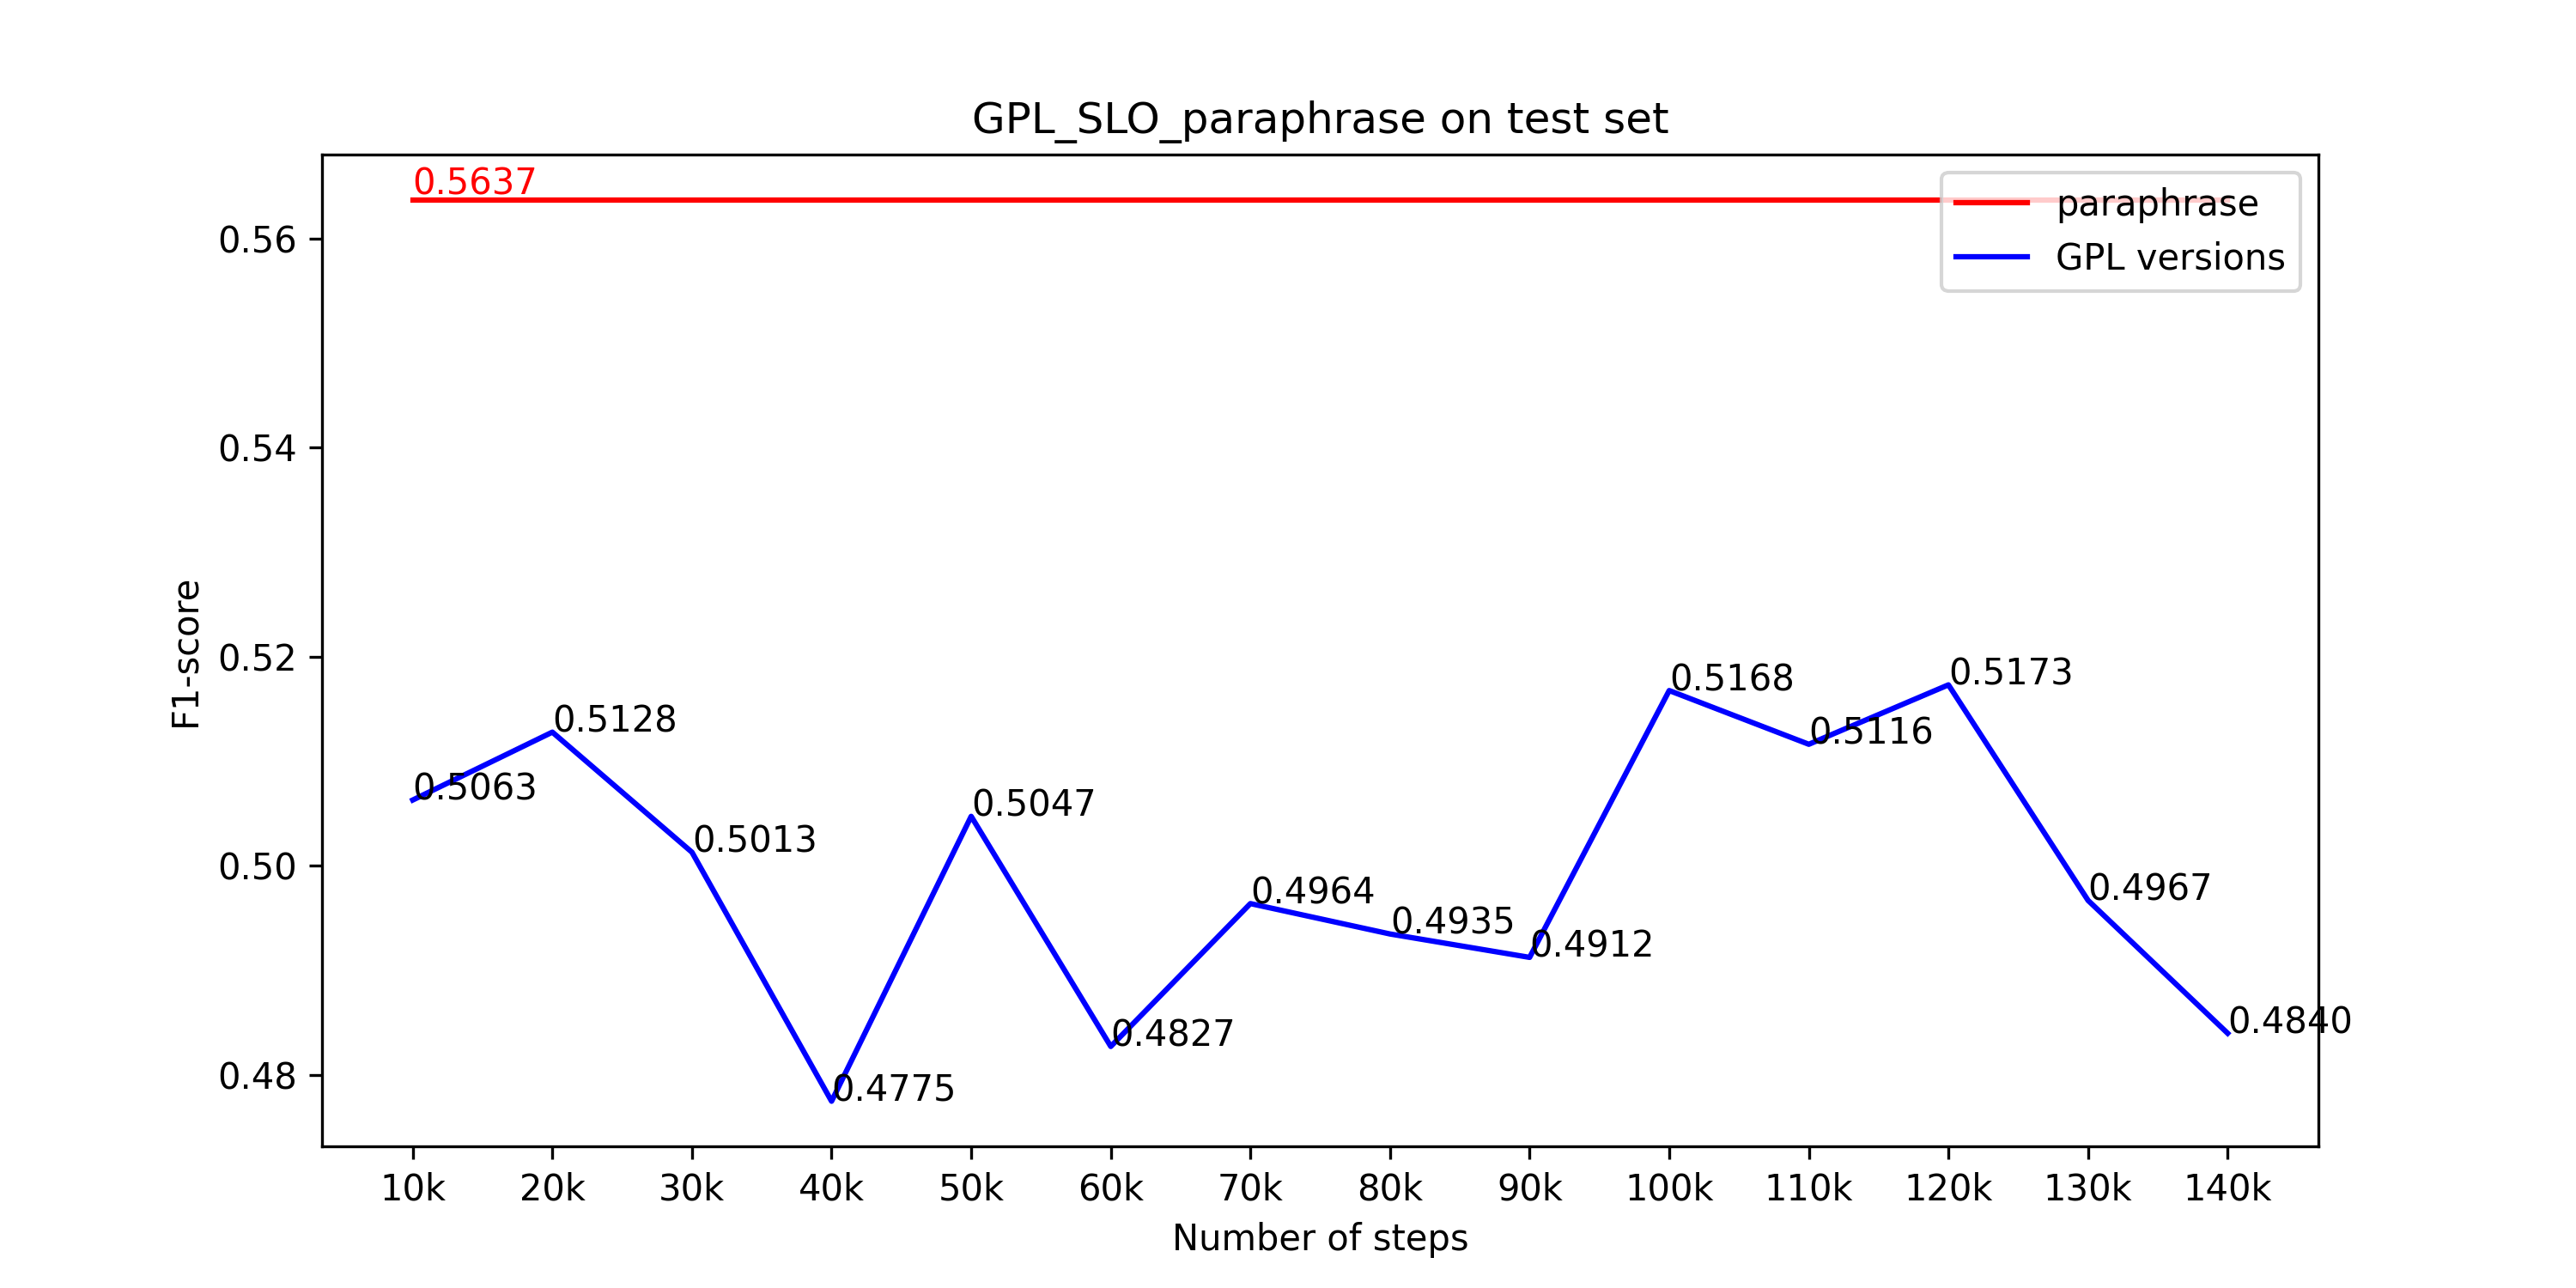
\includegraphics[width=\linewidth]{graphs/GPL_SLO_paraphrase_test.png}
        \caption{F1 score on \textit{test} set evaluated on models, obtained during fine-tuning with the GPL method with {\it slv\_doc2query}~\cite{boshko} for the T5 model.}
		\label{fig:gpl-slo-versions}
    \end{minipage}
\end{figure}

From the graphs, it is evident that the F1 score is lower than the base model for both variants and for all intermediate models. We notice on Figure~\ref{fig:gpl-versions} that lowering the number of steps used for training GPL could result in better performance, but this parameter would have to be chosen carefully and after further testing. The $\text{GPL}_{SLO}$ seems to perform the best at around 100,000 steps, as seen on Figure~\ref{fig:gpl-slo-versions}, but its performance significantly declines at 130,000 and 140,000 steps. Since a similar, though less pronounced, decline is also observed in Figure~\ref{fig:gpl-slo-versions-train} of the training dataset, we are unsure if this is due to just overfitting.


% ---...---...---

\subsection*{\large{2. SloBERTa}}
We decided to also fine-tune and evaluate a different base model, that is {\it SloBERTa}~\cite{sloberta}. The model is monolingual and was trained only on Slovenian datasets. In this section we compared the next models:
\begin{itemize}
	\item base model {\it SloBERTa},
	\item base model fine-tuned with the TSDAE method, trained for 10 epochs - denoted as TSDAE,
	\item base model fine-tuned with the GPL method and {\it msmarco-14langs-mt5-base-v1} \cite{msmarco14langs} for the T5 model - denoted as GPL and
	\item base model fine-tuned with the GPL method and \\{\it slv\_doc2query}~\cite{boshko} for the T5 model - denoted as $\text{GPL}_{SLO}$.
\end{itemize}

As in the case of the {\it paraphrase-multilingual-MiniLM-L12-v2} base model, a new classifier was trained for each of the listed models. Evaluation was once again done on the test set of the SentiNews dataset~\cite{sentiNews}. The results are presented in Table~\ref{tab4}.

\begin{table}[!h]
	\footnotesize
	\begin{center}
		\begin{tabular}{ |l|c|c|c| }
		\hline
		\rowcolor{Blue}Model & Precision & Recall & F1 score\\
		\hline

		Base model & 0.6416 & 0.6209 & \textbf{0.5867}\\
		\hline
		TSDAE & 0.631 & 0.6219 & \textbf{0.5955}\\
		\hline
		GPL & 0.5898 & 0.593 & \textbf{0.5635}\\
		$\text{GPL}_{SLO}$ & 0.5914 & 0.5854 & 0.545\\

		\hline
		\end{tabular}
	\end{center}
\caption{Results of the base model and its fine-tuned variants on the SentiNews dataset~\cite{sentiNews}.}
\label{tab4}
\end{table}

Contrary to the results attained while working with the {\it paraphrase-multilingual-MiniLM-L12-v2} model, where using only the base model achieved the highest F1 score, the {\it SloBERTa} base model is surpassed by its TSDAE fine-tuned variant. The TSDAE model's F1 score is higher than the base model's ({\it SloBERTa}) for 0.0088 or 1.5\%. The improvement is small, but noticable.

Interestingly, the GPL model performs better than the $\text{GPL}_{SLO}$ (the opposite happened with {\it paraphrase-multilingual-MiniLM-L12-v2} model in Table~\ref{tab2}), although the difference between the two is only 3.28\% in F1 score.
Comparing the GPL model to the base model reveals a decrease in the F1 score of 0.0232 or 3,95\%.

Despite the previously used base model {\it paraphrase-\\multilingual-MiniLM-L12-v2} being trained on a training dataset of 50 languages that included Slovenian, the monolingual base model {\it SloBERTa} performs better, as it is solely trained for Slovene. Our sentiment classification problem is done on Slovenian sentences, thus making the {\it SloBERTa} model better suited for our language task. This improved performance is evident when comparing Table~\ref{tab2} with Table~\ref{tab4}. Comparing the scores of the {\it SloBERTa} model, TSDAE and GPL to the {\it paraphrase-multilingual-MiniLM-L12-v2} model (its F1 score of 0.5637 is stated in Table~\ref{tab2}), our observations are:
\begin{itemize}
	\item {\it SloBERTa}'s F1 score is improved by 4.08\%,
	\item TSDAE's F1 score is improved by 5.64\% and
	\item GPL's F1 score is worsened by 0.04\%.
\end{itemize}


\subsection*{Combining the methods}
A combination of the unsupervised adaptation techniques was tested. The approach was to additionally fine-tune the TSDAE model with the GPL method using {\it slv\_doc2query} for the T5 model.

Similarly as with {\it paraphrase-multilingual-MiniLM-L12-v2}, we also considered testing the approach of further fine-tuning the $\text{GPL}_{SLO}$ model using the TSDAE method for 10 epochs, but we were unable to do so because of lack of time. Results of TSDAE+$\text{GPL}_{SLO}$, compared to the base model, are presented in Table~\ref{tab5}.

\begin{table}[!h]
	\footnotesize
	\begin{center}
		\begin{tabular}{ |l|c|c|c| }
		\hline
		\rowcolor{Blue}Model & Precision & Recall & F1 score\\
		\hline

		Base model & 0.6416 & 0.6209 & \textbf{0.5867}\\
		TSDAE+$\text{GPL}_{SLO}$ & 0.5882 & 0.5956 & 0.5784\\
		%$\text{GPL}_{SLO}$+TSDAE & 0.v & 0.v & 0.v\\

		\hline
		\end{tabular}
	\end{center}
\caption{Results of combining the fine-tuning methods TSDAE and GPL on the SentiNews dataset~\cite{sentiNews}.}
\label{tab5}
\end{table}

The combination TSDAE+$\text{GPL}_{SLO}$ does not yield a higher F1 score than the base model. The combination's F1 score is also lower than the TSDAE model's by 0.0171 or 2.87\%, but higher than GPL model's by 0.0149 or 2.64\%. Consequently, it is best to only use the TSDAE fine-tuning method with number of epochs set to 10.


\subsection*{Intermediate models in GPL}
As explained in the case of {\it paraphrase-multilingual-MiniLM-L12-v2} model, we extracted the intermediate models when fine-tuning with the GPL method. A model was saved every 10,000 steps, thus resulting in 13 intermediate and one final model. A classifier was trained for each of the models and evaluated on the train and test set of the SentiNews dataset~\cite{sentiNews}. The results (F1 scores) are shown in Figure~\ref{fig:gpl-sloberta-versions-train} and Figure~\ref{fig:gpl-sloberta-versions} for GPL and in Figure~\ref{fig:gpl-sloberta-slo-versions-train} and Figure~\ref{fig:gpl-sloberta-slo-versions} for $\text{GPL}_{SLO}$.

\begin{figure}
    \centering
    \begin{minipage}{0.5\textwidth}
        \centering
        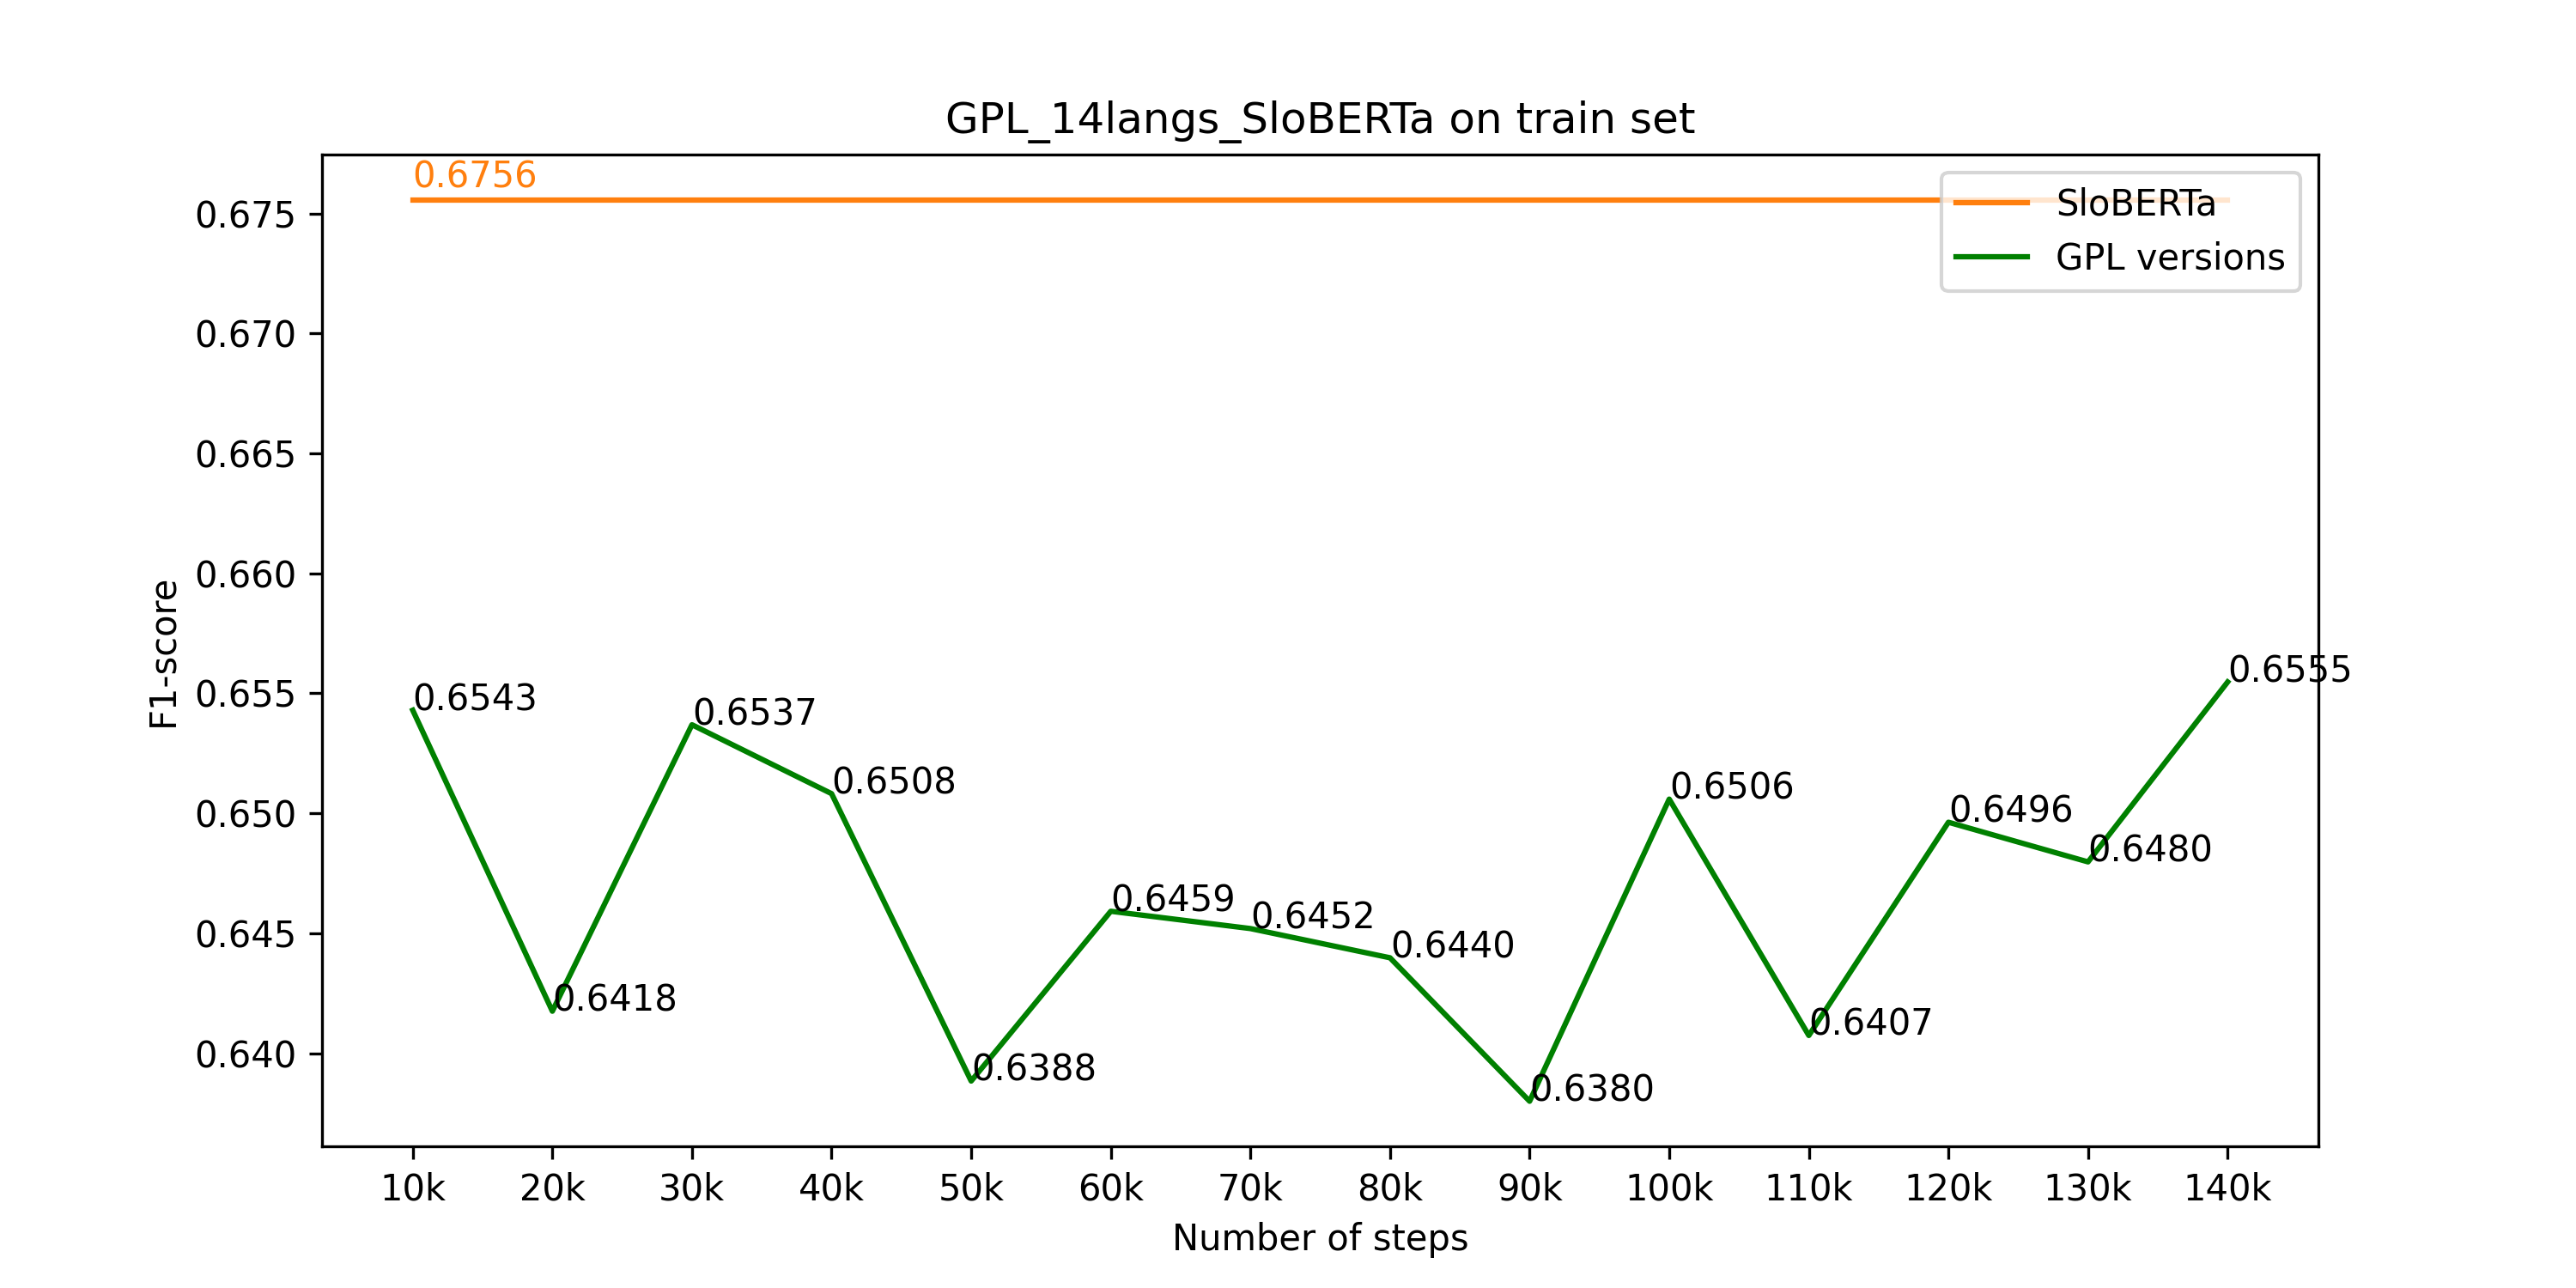
\includegraphics[width=\linewidth]{graphs/GPL_14langs_SloBERTa_train.png}
        \caption{F1 score on \textit{train} set evaluated on models, obtained during fine-tuning with the GPL method with {\it msmarco-14langs-mt5-base-v1}~\cite{msmarco14langs} for the T5 model.}
		\label{fig:gpl-sloberta-versions-train}
    \end{minipage}\hfill
    \begin{minipage}{0.5\textwidth}
        \centering
        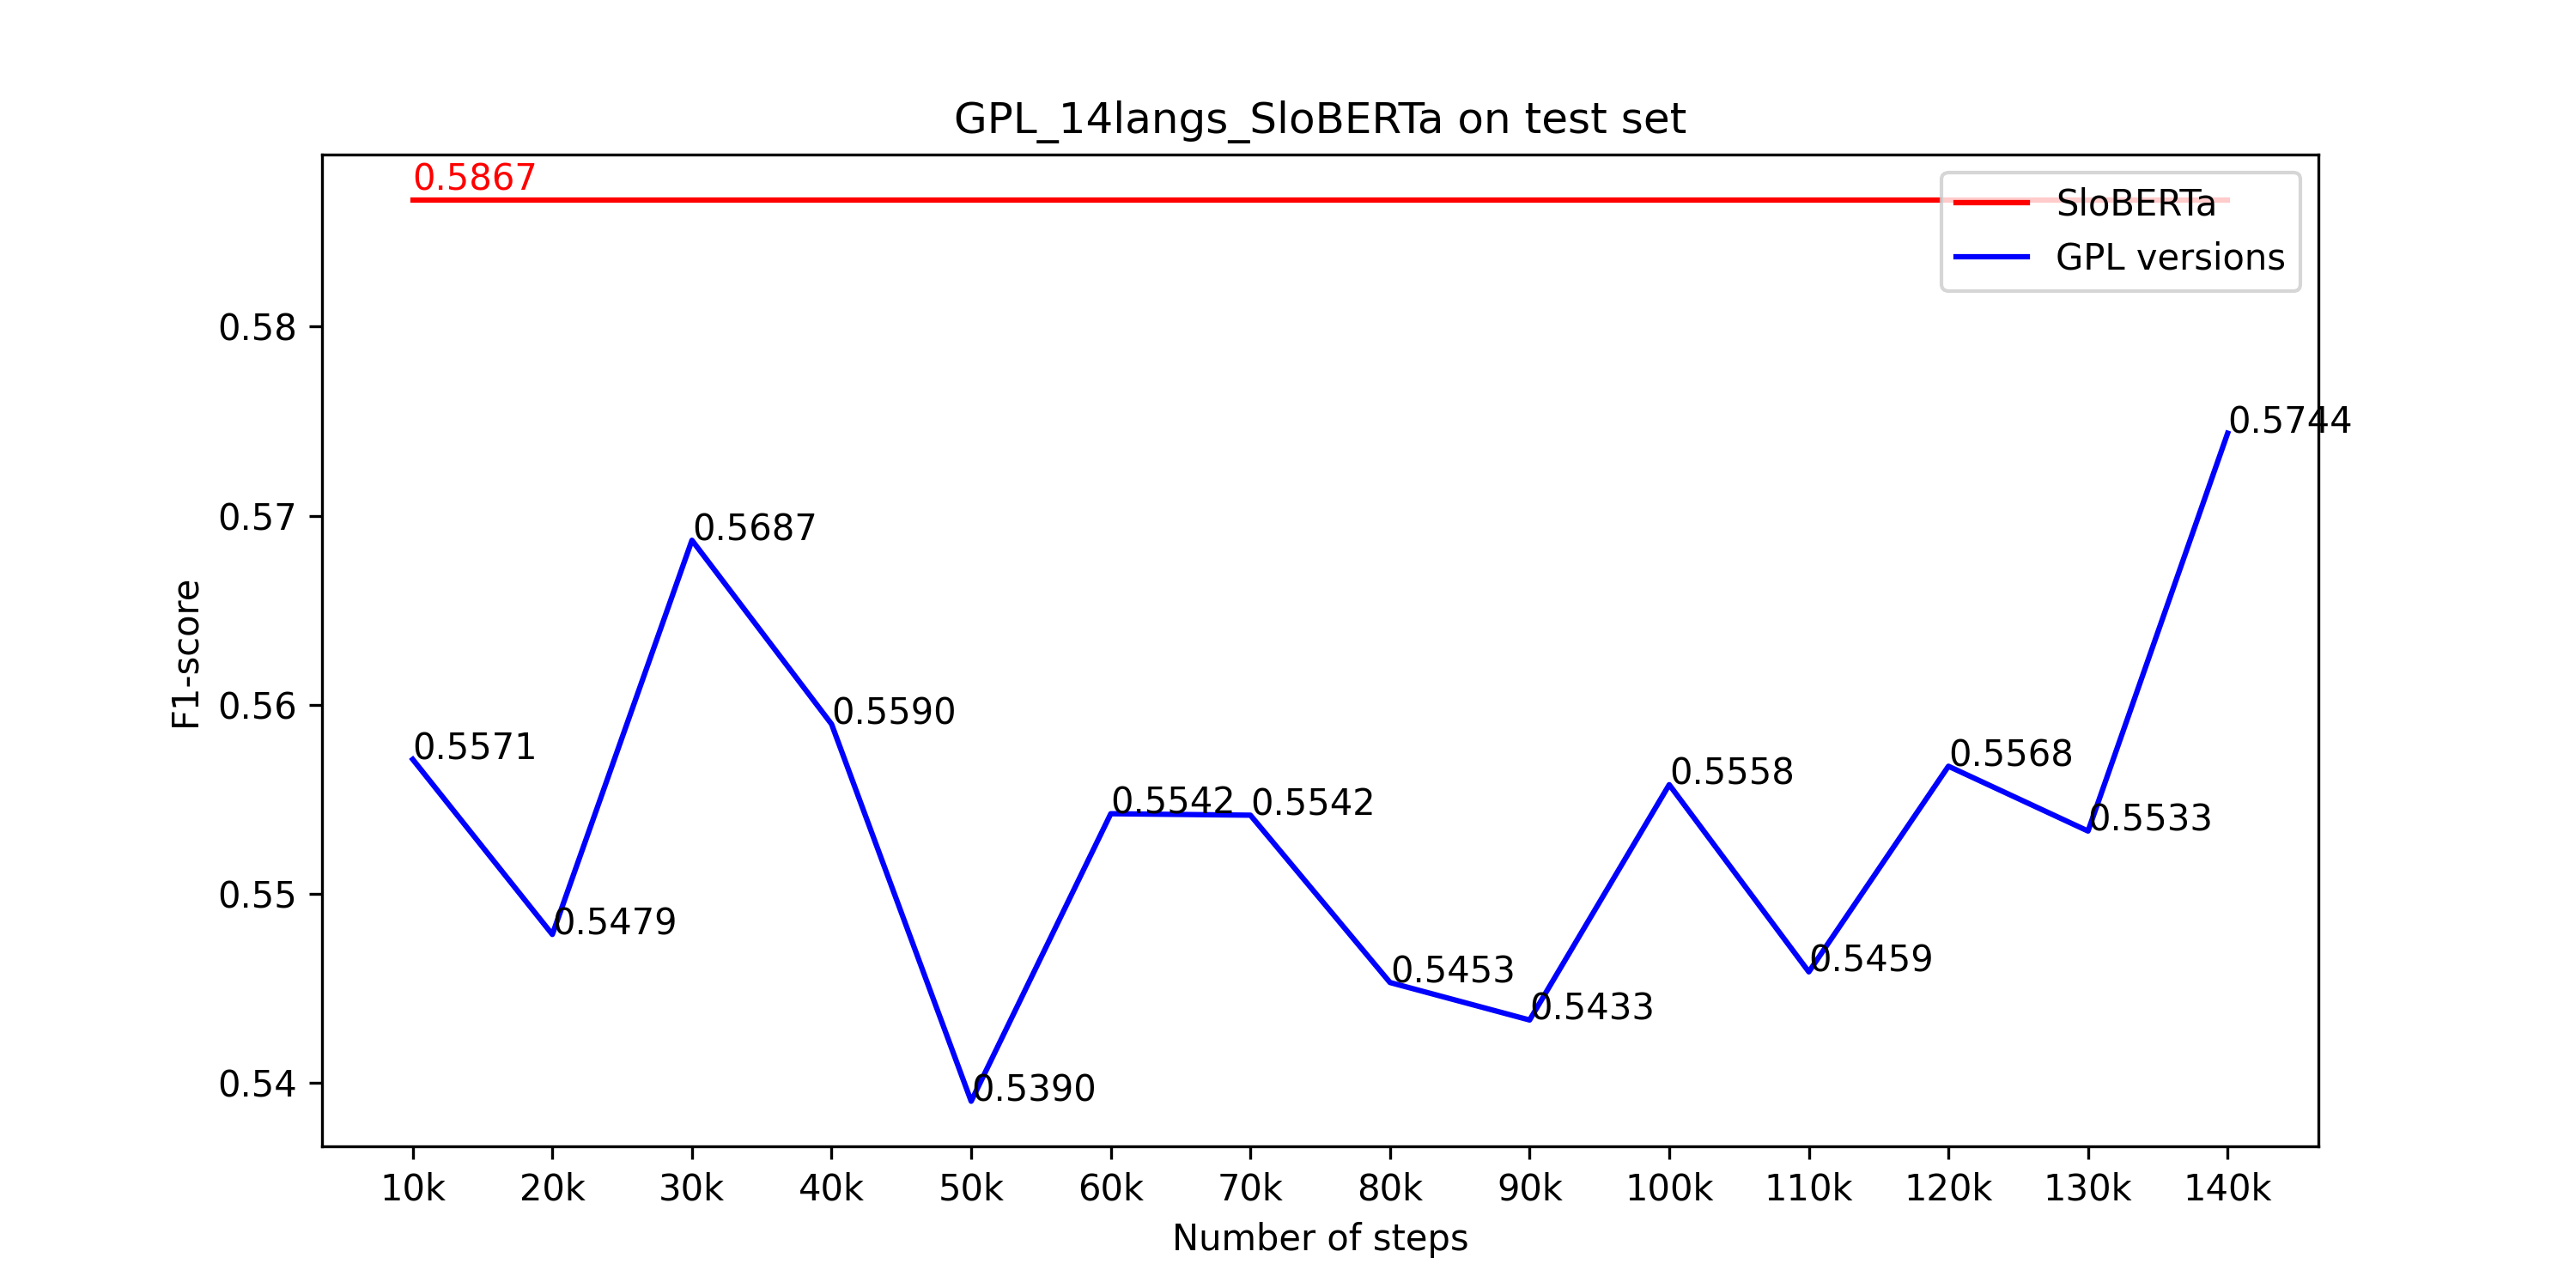
\includegraphics[width=\linewidth]{graphs/GPL_14langs_SloBERTa_test.png}
        \caption{F1 score on \textit{test} set evaluated on models, obtained during fine-tuning with the GPL method with {\it msmarco-14langs-mt5-base-v1}~\cite{msmarco14langs} for the T5 model.}
		\label{fig:gpl-sloberta-versions}
    \end{minipage}
\end{figure}

\begin{figure}
    \centering
    \begin{minipage}{0.5\textwidth}
        \centering
        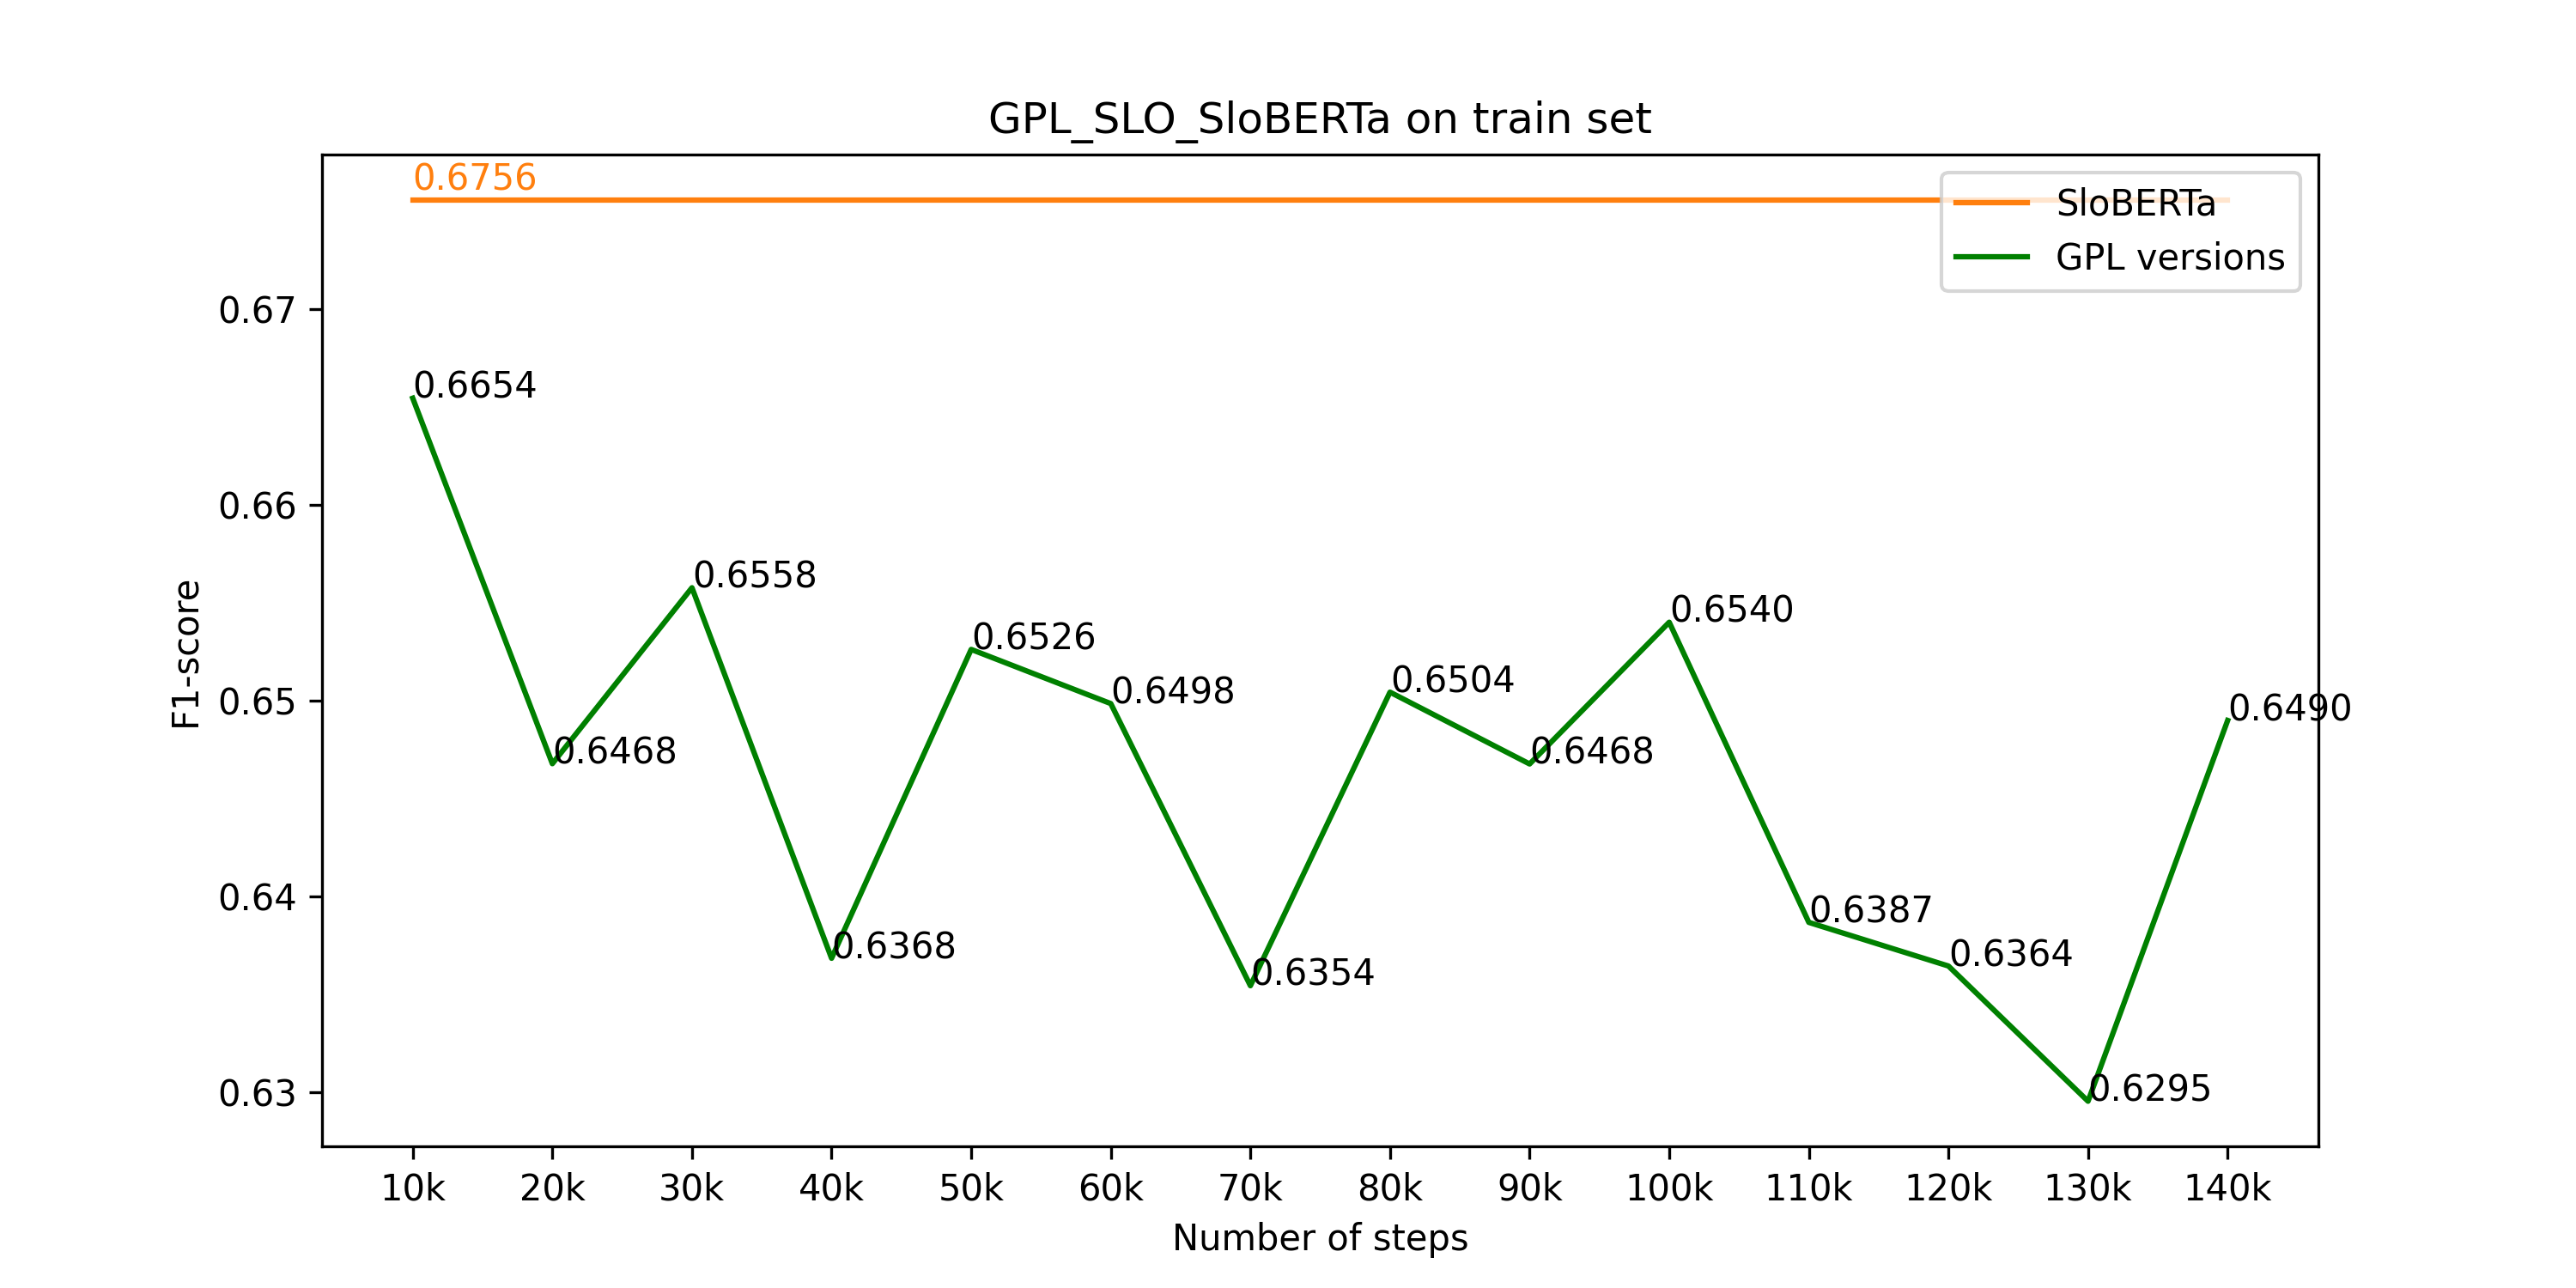
\includegraphics[width=\linewidth]{graphs/GPL_SLO_SloBERTa_train.png}
        \caption{F1 score on \textit{train} set evaluated on models, obtained during fine-tuning with the GPL method with {\it slv\_doc2query}~\cite{boshko} for the T5 model.}
		\label{fig:gpl-sloberta-slo-versions-train}
    \end{minipage}\hfill
    \begin{minipage}{0.5\textwidth}
        \centering
        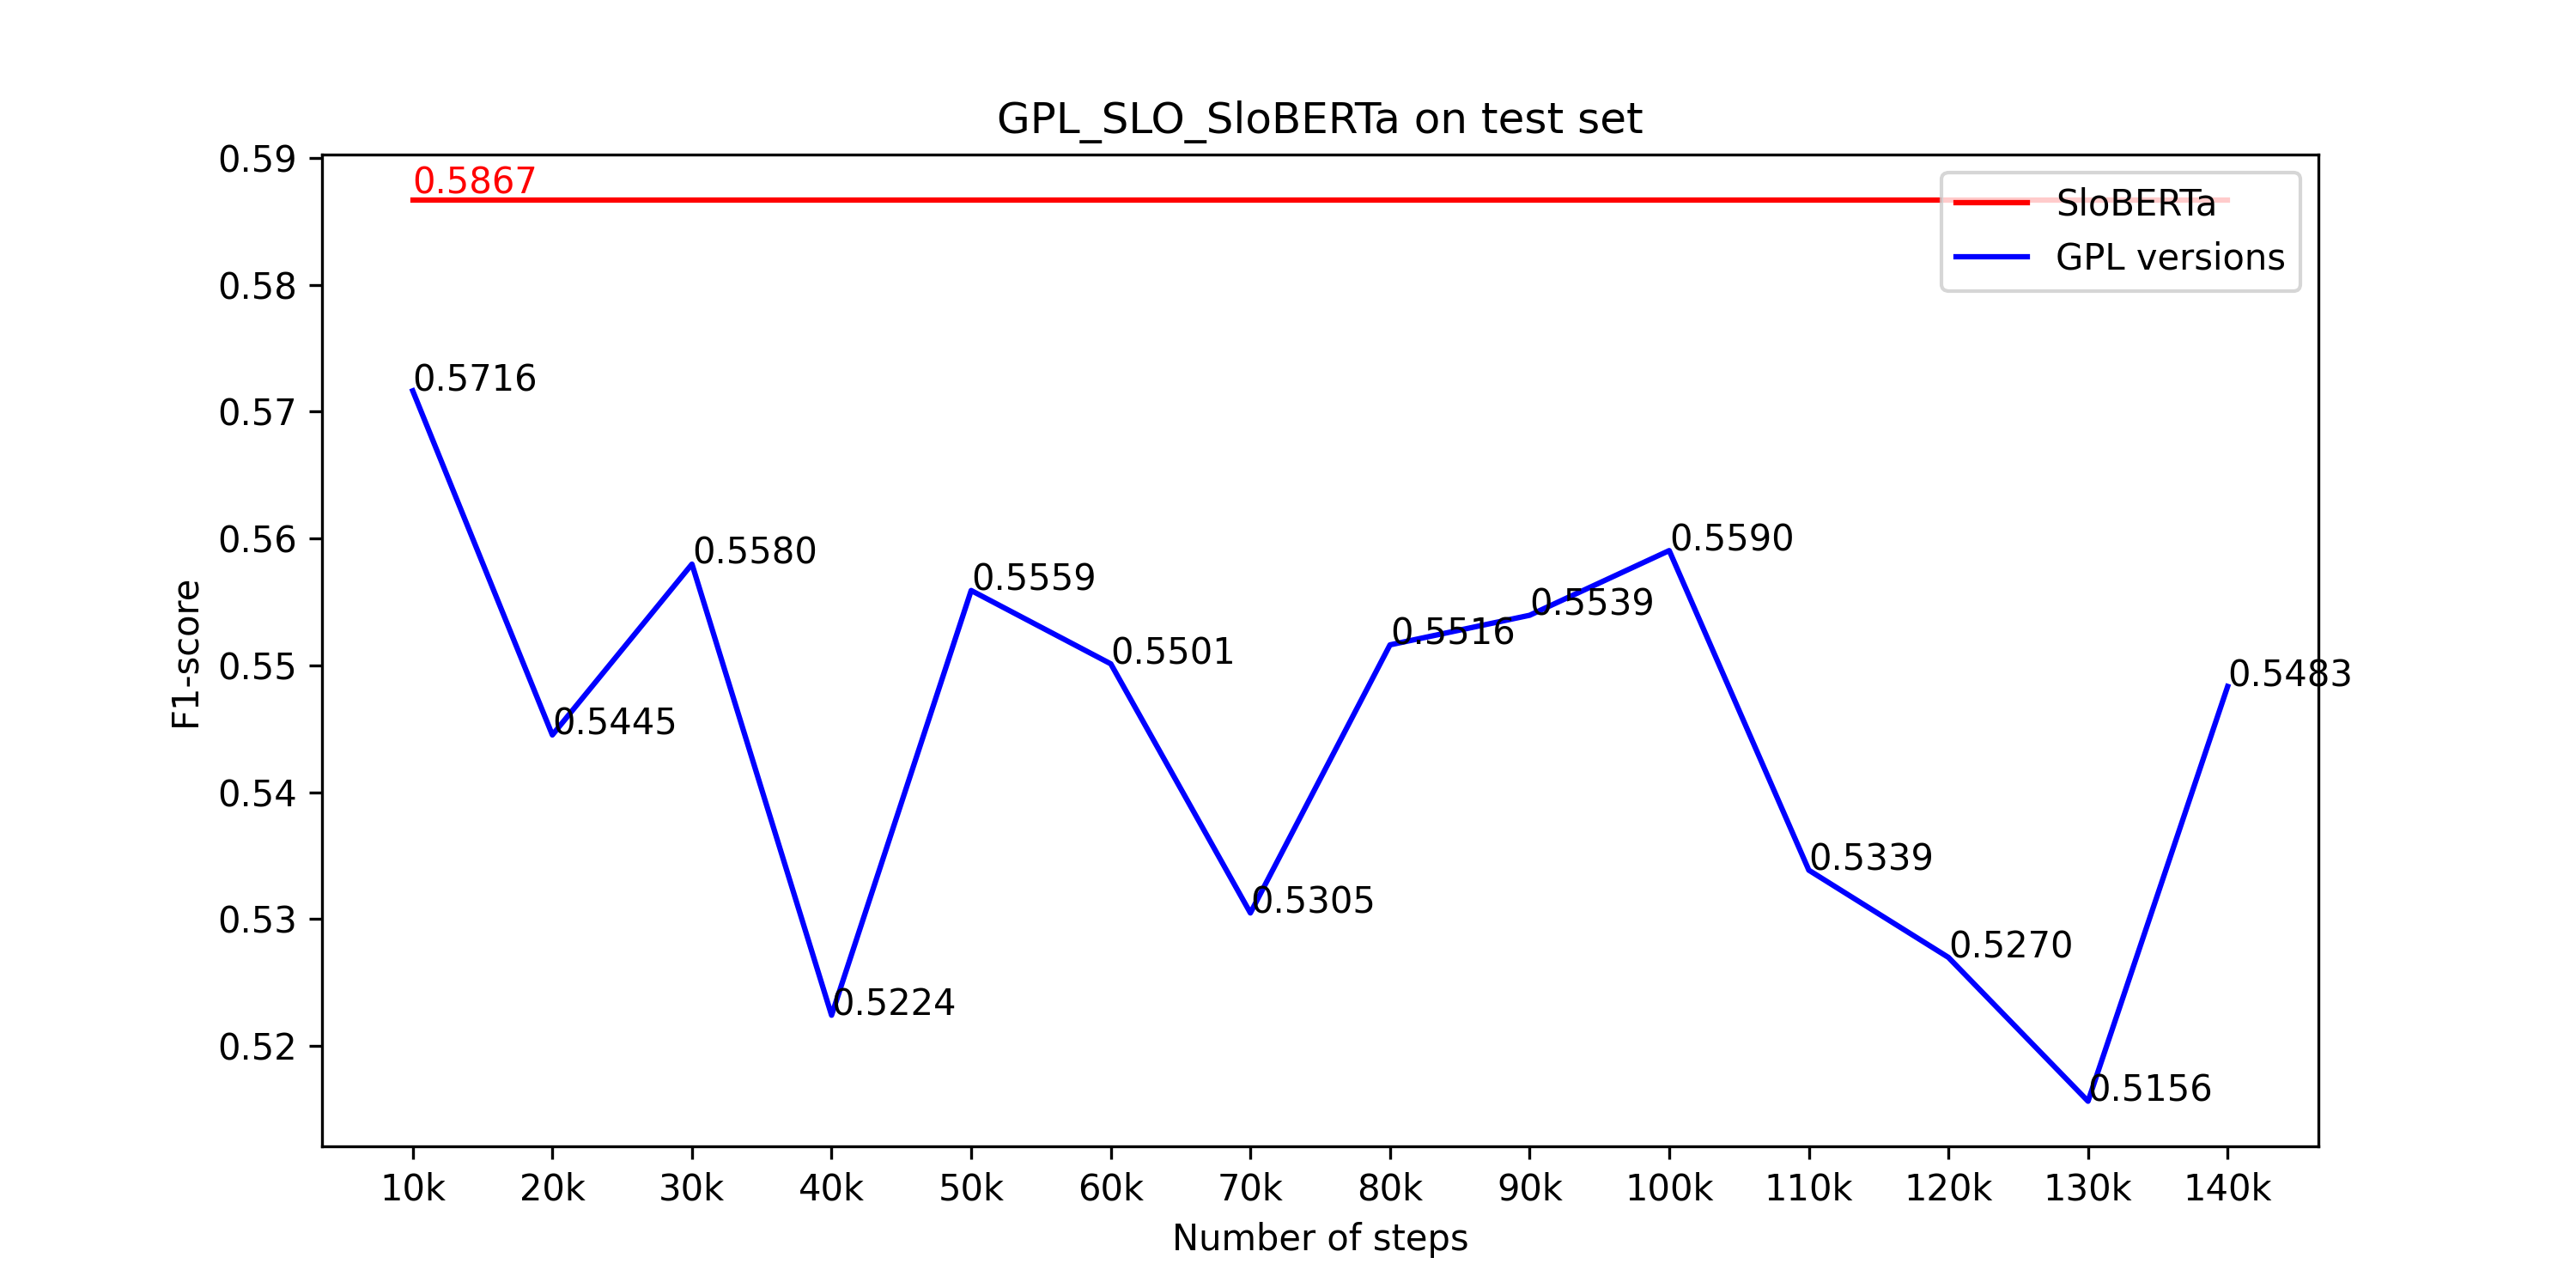
\includegraphics[width=\linewidth]{graphs/GPL_SLO_SloBERTa_test.png}
        \caption{F1 score on \textit{test} set evaluated on models, obtained during fine-tuning with the GPL method with {\it slv\_doc2query}~\cite{boshko} for the T5 model.}
		\label{fig:gpl-sloberta-slo-versions}
    \end{minipage}
\end{figure}

Similarly as before we notice that smaller number of training sets can give us better results than having more steps. We notice that the best F1 score is given by training $\text{GPL}_{SLO}$ for 10,000 steps. This value is almost as good
as the base model F1 score, but doesn't surpass it. Comparing Figure~\ref{fig:gpl-slo-versions} with Figure~\ref{fig:gpl-sloberta-slo-versions}
we clearly see how better our model performs by simply changing the base model.
Training for more than 100,000 steps could probably lead into overfitting based solely on Figure~\ref{fig:gpl-sloberta-slo-versions}, despite the GPL article~\cite{GPL} suggested 140,000 steps, but the model evaluated on the training dataset, as seen on Figure~\ref{fig:gpl-sloberta-slo-versions-train}, once again disputes this fact.
To further check when the model starts to overfit, we should've added more steps to the fine-tuning process, for example something such as 200,000.



%------------------------------------------------



\section*{Discussion}

% Use the Discussion section to objectively evaluate your work, do not just put praise on everything you did, be critical and exposes flaws and weaknesses of your solution. You can also explain what you would do differently if you would be able to start again and what upgrades could be done on the project in the future.

% Ideje:
% - Testiranje na bolj specifičnih domenah.
% - Morda se je bolj smiselno osredotočiti na modele, ki so namenjeni izključno slovenščini.
% - Prilagoditi bi morali korake v GPL, morda še katerega izmed drugih parametrov.
% - Testirati bi morali klasifikator s še kakšnimi drugimi parametri, morda bi ga lahko dlje trenirali in podobno.


The tested unsupervised fine-tuning methods TSDAE and GPL did not perform as well as it was indicated in \cite{wang-etal-2021-tsdae-using} and \cite{GPL} for our Slovenian dataset and sentiment classification problem. The F1 scores we achieved on the test set with the fine-tuned models were almost all lower than the F1 scores of the base models. The only exception was the TSDAE fine-tuned {\it SloBERTa}~\cite{sloberta} model, which improved the base model {\it SloBERTa}'s score by 1.5\%.

Comparing the two base models, {\it paraphrase-multilingual-MiniLM-L12-v2}~\cite{reimers-2019-sentence-bert} and {\it SloBERTa}, we noticed that the latter performs better for sentiment classification of Slovenian sentences. The {\it SloBERTa} base model surpassed the {\it paraphrase-multilingual-MiniLM-L12-v2}'s F1 score by 4.08\%. This is most probably due to {\it SloBERTa} being trained only on Slovenian datasets, while for the {\it paraphrase-multilingual-MiniLM-L12-v2}, the Slovene language was only a part of the training set.

Unfortunately, the combination $\text{GPL}_{SLO}$+TSDAE fine-tuning could not be evaluated for neither of the base models. Comparing it to the combination TSDAE+$\text{GPL}_{SLO}$, that we were able to fine-tune and test, could prove interesting.

The next logical step would be testing the methods on a much more specific domain. The SentiNews dataset was built from different Slovenian news, resulting in a vocabulary that is quite general. If we were to use a very specific dataset, we think that the comparison between the fine-tuned models with TSDAE and GPL method and just the base model might differ from the results achieved in this project.

Since gathering labeled data from specific domains in Slovene language may be sprase, the unsupervised learning we tested could prove useful for such purposes. For example, if we fine-tuned a chosen base model with the TSDAE or GPL method (using {\it msmarco-14langs-mt5-base-v1}~\cite{msmarco14langs} or {\it slv\_doc2query}~\cite{boshko} for the T5 model) on a sentiment dataset, which included Slovene sentences with reviews only for a specific product or range of products in the same category, then the model could potentially achieve better results.

The parameters of the proposed classifier in the project were not tested enough. Further experimenting with the number of epochs and the learning rate could lead us to improved performance. We could also test the difference in performance with changing the GPL parameters, perhaps even testing the method with all of the models it uses for being trained or fine-tuned specifically for the Slovene language.


%------------------------------------------------



\section*{Acknowledgments}

We thank our teaching assistant Boshko Koloski for sharing his expertise on the topic and encouraging our team to explore the tested methods.


%----------------------------------------------------------------------------------------
%	REFERENCE LIST
%----------------------------------------------------------------------------------------
\bibliographystyle{unsrt}
\bibliography{report}


\end{document}
